% Preprint v2: Abstract, Introduction (with related work), Methodology, Experiment and Results, Conclusion.
% Compile with pdflatex (twice) or on Overleaf with the whole report/ folder.
\documentclass[10pt,a4paper]{article}

\usepackage[utf8]{inputenc}
\usepackage[T1]{fontenc}
\usepackage[english]{babel}
\usepackage{lmodern}
\usepackage{microtype}
\usepackage[margin=2cm]{geometry}
\usepackage{booktabs}
\usepackage{graphicx}
\usepackage{caption}
\usepackage{amsmath}
\usepackage[hidelinks]{hyperref}

\captionsetup{font=small,labelfont=bf}
\graphicspath{{figures/}}
% Generated by scripts/18_preprint_package.py from the result files; do not edit by hand.
% Use the macros in the text, so every number follows the results (e.g. \resHOneBConsensusOr).
\newcommand{\resPending}{\textit{[czeka na H1-A]}}
\newcommand{\resWaiting}{\textit{[czeka na dane]}}
\newcommand{\resRedditFrame}{62\,636}
\newcommand{\resRedditPilot}{32}
\newcommand{\resRedditPilotTwo}{30}
\newcommand{\resRedditDev}{148}
\newcommand{\resRedditTest}{320}
\newcommand{\resRedditCodedDev}{78}
\newcommand{\resRedditCodedTest}{78}
\newcommand{\resRedditTestCiting}{68}
\newcommand{\resWikipediaFrame}{1453}
\newcommand{\resWikipediaPilot}{21}
\newcommand{\resWikipediaPilotTwo}{30}
\newcommand{\resWikipediaDev}{152}
\newcommand{\resWikipediaTest}{327}
\newcommand{\resWikipediaCodedDev}{147}
\newcommand{\resWikipediaCodedTest}{147}
\newcommand{\resWikipediaTestCiting}{20}
\newcommand{\resGoldLabelsIS}{200}
\newcommand{\resGoldLabelsJP}{250}
\newcommand{\resPilotRedditCitesAlpha}{$-$0{,}03 [$-$0{,}09; 0{,}00]}
\newcommand{\resPilotRedditCitesAgreement}{0{,}91}
\newcommand{\resPilotRedditMasiAlpha}{0{,}34 [0{,}11; 0{,}54]}
\newcommand{\resPilotRedditMasiAgreement}{0{,}50}
\newcommand{\resPilotWikipediaCitesAlpha}{$-$0{,}05 [$-$0{,}14; 0{,}00]}
\newcommand{\resPilotWikipediaCitesAgreement}{0{,}86}
\newcommand{\resPilotWikipediaEditAlpha}{0{,}70 [$-$0{,}02; 1{,}00]}
\newcommand{\resPilotWikipediaEditAgreement}{0{,}90}
\newcommand{\resPilotWikipediaMasiAlpha}{$-$0{,}03 [$-$0{,}12; 0{,}00]}
\newcommand{\resPilotWikipediaMasiAgreement}{0{,}86}
\newcommand{\resPilotRedditUnits}{32}
\newcommand{\resPilotWikipediaUnits}{21}
\newcommand{\resPilotDisputes}{20}
\newcommand{\resPilotRedditISCitingShare}{100\,\%}
\newcommand{\resTestRulesRedditCitesF}{0{,}10 [0{,}00; 0{,}20]}
\newcommand{\resTestRulesRedditCitesKappa}{$-$0{,}01}
\newcommand{\resTestRulesRedditMasi}{0{,}18 [0{,}09; 0{,}27]}
\newcommand{\resTestRulesWikipediaCitesF}{0{,}09 [0{,}03; 0{,}19]}
\newcommand{\resTestRulesWikipediaCitesKappa}{$-$0{,}03}
\newcommand{\resTestRulesWikipediaMasi}{0{,}70 [0{,}62; 0{,}77]}
\newcommand{\resTestRulesRedditMacroF}{0{,}08 [0{,}00; 0{,}16]}
\newcommand{\resTestZeroshotRedditCitesF}{0{,}90 [0{,}83; 0{,}95]}
\newcommand{\resTestZeroshotRedditCitesKappa}{0{,}15}
\newcommand{\resTestZeroshotRedditMasi}{0{,}32 [0{,}22; 0{,}42]}
\newcommand{\resTestZeroshotWikipediaCitesF}{0{,}17 [0{,}05; 0{,}31]}
\newcommand{\resTestZeroshotWikipediaCitesKappa}{$-$0{,}01}
\newcommand{\resTestZeroshotWikipediaMasi}{0{,}61 [0{,}49; 0{,}73]}
\newcommand{\resTestZeroshotRedditMacroF}{0{,}42 [0{,}26; 0{,}54]}
\newcommand{\resTestGlinerRedditCitesF}{0{,}96 [0{,}92; 0{,}99]}
\newcommand{\resTestGlinerRedditCitesKappa}{0{,}54}
\newcommand{\resTestGlinerRedditMasi}{0{,}46 [0{,}35; 0{,}57]}
\newcommand{\resTestGlinerWikipediaCitesF}{0{,}26 [0{,}06; 0{,}51]}
\newcommand{\resTestGlinerWikipediaCitesKappa}{0{,}27}
\newcommand{\resTestGlinerWikipediaMasi}{0{,}85 [0{,}77; 0{,}92]}
\newcommand{\resTestGlinerRedditMacroF}{0{,}68 [0{,}43; 0{,}78]}
\newcommand{\resTestZeroshotWikipediaEditF}{0{,}37 [0{,}26; 0{,}48]}
\newcommand{\resTestGlinerRedditCitesPrecision}{0{,}93}
\newcommand{\resTestGlinerRedditCitesRecall}{1{,}00}
\newcommand{\resTestGlinerRedditMediaF}{0{,}66}
\newcommand{\resTestGlinerRedditSocialBlogF}{0{,}70}
\newcommand{\resTestGlinerRedditMasiIS}{0{,}29}
\newcommand{\resTestGlinerWikipediaCitesFIS}{0{,}11}
\newcommand{\resTestGlinerRedditMasiJP}{0{,}61}
\newcommand{\resTestGlinerWikipediaCitesFJP}{0{,}56}
\newcommand{\resDevGlinerRedditMasi}{0{,}50}
\newcommand{\resDevRulesvtwoRedditMasi}{0{,}60}
\newcommand{\resDevRulesvtwoWikipediaEditF}{0{,}80}
\newcommand{\resDevRefsWikipediaEditF}{0{,}57}
\newcommand{\resMcnemarRedditZeroshotGlinerOnlyFirst}{0}
\newcommand{\resMcnemarRedditZeroshotGlinerOnlySecond}{7}
\newcommand{\resMcnemarRedditZeroshotGlinerP}{0{,}016}
\newcommand{\resMcnemarWikipediaZeroshotGlinerOnlyFirst}{5}
\newcommand{\resMcnemarWikipediaZeroshotGlinerOnlySecond}{39}
\newcommand{\resMcnemarWikipediaZeroshotGlinerP}{$<$0{,}001}
\newcommand{\resMcnemarRedditVoneGlinerOnlyFirst}{6}
\newcommand{\resMcnemarRedditVoneGlinerOnlySecond}{66}
\newcommand{\resMcnemarRedditVoneGlinerP}{$<$0{,}001}
\newcommand{\resTauGlinerReddit}{0{,}55}
\newcommand{\resTauGlinerRedditP}{0{,}061}
\newcommand{\resGoldShareRedditCitesSource}{0{,}88 [0{,}81; 0{,}93]}
\newcommand{\resGoldShareRedditMedia}{0{,}41 [0{,}33; 0{,}49]}
\newcommand{\resGoldShareRedditSocialBlog}{0{,}33 [0{,}25; 0{,}41]}
\newcommand{\resGoldShareWikipediaCitesSource}{0{,}13 [0{,}09; 0{,}19]}
\newcommand{\resGoldShareWikipediaPersonal}{0{,}05 [0{,}02; 0{,}10]}
\newcommand{\resErrorsVoneTotal}{127}
\newcommand{\resErrorsGlinerTotal}{88}
\newcommand{\resErrorsRulesvtwoTotal}{97}
\newcommand{\resErrorsVoneUrl}{71}
\newcommand{\resErrorsVoneUrlShare}{56\,\%}
\newcommand{\resDifferentialGlinerRedditPeriodFpP}{0{,}056}
\newcommand{\resDifferentialGlinerRedditSubredditFpP}{0{,}006}
\newcommand{\resHoneSample}{6240}
\newcommand{\resHoneBCiting}{5154}
\newcommand{\resHoneBConsensusOr}{1{,}03 [0{,}99; 1{,}06]}
\newcommand{\resHoneBConsensusP}{0{,}928}
\newcommand{\resHoneBAlternativeOr}{0{,}99 [0{,}97; 1{,}01]}
\newcommand{\resHoneBAlternativeP}{0{,}853}
\newcommand{\resHoneBConsensusTwentyOr}{1{,}04 [1{,}01; 1{,}08]}
\newcommand{\resHoneBConsensusTwentyP}{0{,}994}
\newcommand{\resHoneBAlternativeTwentyOr}{0{,}99 [0{,}98; 1{,}01]}
\newcommand{\resHoneBAlternativeTwentyP}{0{,}759}
\newcommand{\resHoneBConsensusScienceOr}{1{,}03 [0{,}99; 1{,}07]}
\newcommand{\resHoneBConsensusScienceP}{0{,}949}
\newcommand{\resHoneBAlternativeScienceOr}{0{,}99 [0{,}96; 1{,}02]}
\newcommand{\resHoneBAlternativeScienceP}{0{,}829}
\newcommand{\resHoneBConsensusConspiracyOr}{1{,}01 [0{,}90; 1{,}14]}
\newcommand{\resHoneBConsensusConspiracyP}{0{,}577}
\newcommand{\resHoneBAlternativeConspiracyOr}{1{,}00 [0{,}95; 1{,}04]}
\newcommand{\resHoneBAlternativeConspiracyP}{0{,}592}
\newcommand{\resHoneBConsensusShareTwothousandsix}{22\,\%}
\newcommand{\resHoneBConsensusShareLateLow}{10\,\%}
\newcommand{\resHoneBConsensusShareLateHigh}{14\,\%}
\newcommand{\resHoneBAlternativeShareTwothousandfive}{35\,\%}
\newcommand{\resHoneBAlternativeShareLateHigh}{47\,\%}
\newcommand{\resHoneConspiracyShareTwothousandeight}{2\,\%}
\newcommand{\resHoneConspiracyShareTwothousandeighteen}{58\,\%}
\newcommand{\resHoneBConsensusShiftTotal}{$-$3{,}7\,pp}
\newcommand{\resHoneBConsensusShiftWithin}{2{,}7\,pp}
\newcommand{\resHoneBConsensusShiftComposition}{$-$6{,}5\,pp}
\newcommand{\resHoneBAlternativeShiftTotal}{7{,}6\,pp}
\newcommand{\resHoneBAlternativeShiftWithin}{0{,}2\,pp}
\newcommand{\resHoneBAlternativeShiftComposition}{7{,}3\,pp}
\newcommand{\resHtwoBeforeReviewOr}{1{,}47 [1{,}09; 1{,}99]}
\newcommand{\resHtwoBeforeReviewP}{0{,}006}
\newcommand{\resHtwoLinks}{1341}
\newcommand{\resHtwoAlternativeLinks}{10}
\newcommand{\resHtwoModelLinks}{1207}
\newcommand{\resHtwoAlternativePages}{2}
\newcommand{\resHtwoOfficialLinks}{8}
\newcommand{\resHtwoWhoRepeats}{6}
\newcommand{\resHtwoByOwnerLinks}{2}
\newcommand{\resHtwoOr}{1{,}47 [1{,}09; 1{,}99]}
\newcommand{\resHtwoP}{0{,}006}
\newcommand{\resHtwoWithoutCovidOr}{1{,}39 [0{,}83; 2{,}33]}
\newcommand{\resHtwoWithoutCovidP}{0{,}105}
\newcommand{\resHtwoWithoutTwentytwentyOr}{1{,}36 [0{,}78; 2{,}37]}
\newcommand{\resHtwoWithoutTwentytwentyP}{0{,}138}
\newcommand{\resHtwoClassifiedOr}{1{,}47 [1{,}09; 1{,}99]}
\newcommand{\resHtwoClassifiedP}{0{,}006}
\newcommand{\resHtwoPermutationP}{0{,}070}
\newcommand{\resHtwoFirthOr}{1{,}43 [1{,}01; 2{,}02]}
\newcommand{\resHtwoFirthP}{0{,}006}
\newcommand{\resHtwoFirthEvents}{10}
\newcommand{\resHtwoFirstOr}{1{,}59 [0{,}99; 2{,}55]}
\newcommand{\resHtwoFirstP}{0{,}009}
\newcommand{\resHtwoFirstEvents}{4}
\newcommand{\resHtwoOwnerOr}{1{,}31 [0{,}85; 2{,}04]}
\newcommand{\resHtwoOwnerP}{0{,}027}
\newcommand{\resHtwoOwnerEvents}{2}
\newcommand{\resHtwoExactP}{0{,}205}
\newcommand{\resHoneAPilotUnits}{\textit{nie zakodowano}}
\newcommand{\resHoneAPilotAlpha}{\textit{nie zakodowano}}
\newcommand{\resHoneAPilotKappa}{\textit{nie zakodowano}}
\newcommand{\resHoneAPilotAgreement}{\textit{nie zakodowano}}
\newcommand{\resHoneADevPosts}{218}
\newcommand{\resHoneADevChallengesF}{0{,}25}
\newcommand{\resHoneADevKappa}{0{,}33}
\newcommand{\resHoneADevMacroF}{0{,}45}
\newcommand{\resHoneADevAccuracy}{0{,}83}
\newcommand{\resHoneATestPosts}{216}
\newcommand{\resHoneATestChallengesF}{0{,}33}
\newcommand{\resHoneATestKappa}{0{,}24}
\newcommand{\resHoneATestMacroF}{0{,}44}
\newcommand{\resHoneATestAccuracy}{0{,}80}
\newcommand{\resHoneAGate}{niespełniony}
\newcommand{\resHoneAThresholds}{relevance 0{,}30, supports 0{,}30, challenges 0{,}70}
\newcommand{\resHoneAChallengesOr}{\textit{nie testowano}}
\newcommand{\resHoneAChallengesP}{\textit{nie testowano}}
\newcommand{\resHoneASupportsOr}{\textit{nie testowano}}
\newcommand{\resHoneASupportsP}{\textit{nie testowano}}
\newcommand{\resHoneAChallengesTwentyOr}{\textit{nie testowano}}
\newcommand{\resHoneAChallengesTwentyP}{\textit{nie testowano}}
\newcommand{\resHoneASupportsTwentyOr}{\textit{nie testowano}}
\newcommand{\resHoneASupportsTwentyP}{\textit{nie testowano}}
\newcommand{\resHoneAChallengesScienceOr}{\textit{nie testowano}}
\newcommand{\resHoneAChallengesScienceP}{\textit{nie testowano}}
\newcommand{\resHoneASupportsScienceOr}{\textit{nie testowano}}
\newcommand{\resHoneASupportsScienceP}{\textit{nie testowano}}
\newcommand{\resHoneAChallengesConspiracyOr}{\textit{nie testowano}}
\newcommand{\resHoneAChallengesConspiracyP}{\textit{nie testowano}}
\newcommand{\resHoneASupportsConspiracyOr}{\textit{nie testowano}}
\newcommand{\resHoneASupportsConspiracyP}{\textit{nie testowano}}
\newcommand{\resHoneARelevantPosts}{\textit{nie testowano}}
\newcommand{\resHoneAChallengesShareEarly}{\textit{nie testowano}}
\newcommand{\resHoneAChallengesShareLate}{\textit{nie testowano}}
\newcommand{\resHoneAStatus}{warunek trafności niespełniony: H1-A niemierzalne instrumentem \kod{stance\_v1}}
\newcommand{\resEnrichedPosts}{277}
\newcommand{\resEnrichedTopic}{67}
\newcommand{\resEnrichedScience}{150}
\newcommand{\resEnrichedRest}{60}
\newcommand{\resStanceDevChallengesPosts}{50}
\newcommand{\resStanceTestChallengesPosts}{42}
\newcommand{\resPlanCAiChecked}{335}
\newcommand{\resPlanCAiChanged}{0\,\%}
\newcommand{\resPlanCCheckedBy}{ludzi}
\newcommand{\resPlanCStanceAutoShare}{23\,\%}
\newcommand{\resPlanCStanceControls}{11}
\newcommand{\resPlanCStanceRulePrecision}{11/11}
\newcommand{\resPlanCSourcesAutoShare}{4\,\%}
\newcommand{\resPlanCSourcesControls}{1}
\newcommand{\resPlanCSourcesRulePrecision}{1/1}
\newcommand{\resPlanCErrorsAutoShare}{22\,\%}
\newcommand{\resPlanCErrorsControls}{9}
\newcommand{\resPlanCErrorsRulePrecision}{9/9}
\newcommand{\resPlanCDomainsAutoShare}{54\,\%}
\newcommand{\resPlanCDomainsControls}{20}
\newcommand{\resPlanCDomainsRulePrecision}{19/20}
\newcommand{\resHoneATestChallengesPrecision}{0{,}80}
\newcommand{\resHoneATestChallengesRecall}{0{,}21}
\newcommand{\resHoneATestAllRowsChallengesF}{0{,}33}
\newcommand{\resHoneATestAllRowsKappa}{0{,}27}
\newcommand{\resHoneAReviewedPosts}{171}
\newcommand{\resAuditConsensusJ}{0{,}20 [$-$0{,}01; 0{,}55]}
\newcommand{\resAuditConsensusSensitivity}{0{,}35}
\newcommand{\resAuditConsensusSpecificity}{0{,}85}
\newcommand{\resAuditConsensusValid}{tylko opis}
\newcommand{\resAuditConsensusPositives}{26}
\newcommand{\resAuditAlternativeJ}{0{,}59 [0{,}44; 0{,}71]}
\newcommand{\resAuditAlternativeSensitivity}{0{,}81}
\newcommand{\resAuditAlternativeSpecificity}{0{,}77}
\newcommand{\resAuditAlternativeValid}{ważny}
\newcommand{\resAuditAlternativePositives}{76}
\newcommand{\resControlStanceKappa}{0{,}84}
\newcommand{\resControlStanceKappaN}{84}
\newcommand{\resControlStanceAgreement}{90\,\% [82; 95]}
\newcommand{\resControlStanceAgreementN}{84}
\newcommand{\resControlChallengesKept}{87\,\% [75; 94]}
\newcommand{\resControlChallengesKeptN}{47}
\newcommand{\resControlAuditExact}{87\,\% [70; 95]}
\newcommand{\resControlAuditExactN}{30}
\newcommand{\resControlSourcesExact}{93\,\% [79; 98]}
\newcommand{\resControlSourcesExactN}{30}
\newcommand{\resControlSourcesPilotExact}{100\,\% [81; 100]}
\newcommand{\resControlSourcesPilotExactN}{16}
\newcommand{\resControlSourcesGoldExact}{86\,\% [60; 96]}
\newcommand{\resControlSourcesGoldExactN}{14}

% Generated by scripts/28_preprint_v2_package.py from the result files; do not edit by hand.
% Use the macros in the text, so every number follows the results (e.g. \resHOneBConsensusOr).
\newcommand{\resESrcARedditFOne}{0.93 [0.89, 0.97]}
\newcommand{\resESrcARedditMasi}{0.62 [0.52, 0.71]}
\newcommand{\resESrcAWikipediaFOne}{0.29 [0.10, 0.46]}
\newcommand{\resESrcAWikipediaMasi}{0.79 [0.73, 0.86]}
\newcommand{\resESrcAWikipediaMissed}{28}
\newcommand{\resESrcAPersonalKappa}{0.00}
\newcommand{\resESrcAUncertain}{19\%}
\newcommand{\resESrcBRedditFOne}{0.94 [0.90, 0.97]}
\newcommand{\resESrcBRedditMasi}{0.61 [0.51, 0.70]}
\newcommand{\resESrcBWikipediaFOne}{0.32 [0.14, 0.49]}
\newcommand{\resESrcBWikipediaMasi}{0.79 [0.73, 0.86]}
\newcommand{\resESrcBWikipediaMissed}{27}
\newcommand{\resESrcBPersonalKappa}{$-$0.01}
\newcommand{\resESrcBUncertain}{23\%}
\newcommand{\resESrcCRedditFOne}{0.98 [0.96, 1.00]}
\newcommand{\resESrcCRedditMasi}{0.66 [0.57, 0.75]}
\newcommand{\resESrcCWikipediaFOne}{0.66 [0.50, 0.78]}
\newcommand{\resESrcCWikipediaMasi}{0.84 [0.78, 0.90]}
\newcommand{\resESrcCWikipediaMissed}{14}
\newcommand{\resESrcCPersonalKappa}{0.58}
\newcommand{\resESrcCUncertain}{25\%}
\newcommand{\resESrcDRedditFOne}{0.98 [0.96, 1.00]}
\newcommand{\resESrcDRedditMasi}{0.65 [0.55, 0.74]}
\newcommand{\resESrcDWikipediaFOne}{0.62 [0.46, 0.75]}
\newcommand{\resESrcDWikipediaMasi}{0.82 [0.76, 0.88]}
\newcommand{\resESrcDWikipediaMissed}{14}
\newcommand{\resESrcDPersonalKappa}{0.51}
\newcommand{\resESrcDUncertain}{27\%}
\newcommand{\resESrcABCitesKappa}{0.96 [0.92, 0.99]}
\newcommand{\resESrcABTypesAlphaMasi}{0.94 [0.91, 0.98]}
\newcommand{\resESrcABEditKappa}{0.95 [0.88, 1.00]}
\newcommand{\resESrcCDCitesKappa}{0.96 [0.92, 0.99]}
\newcommand{\resESrcCDTypesAlphaMasi}{0.95 [0.91, 0.98]}
\newcommand{\resESrcCDEditKappa}{0.98 [0.92, 1.00]}
\newcommand{\resESrcCodebookShiftKappaMin}{0.74}
\newcommand{\resESrcCodebookShiftKappaMax}{0.79}
\newcommand{\resESrcMcnemarACFixed}{14}
\newcommand{\resESrcMcnemarACBroken}{5}
\newcommand{\resESrcMcnemarACP}{0.064}
\newcommand{\resESrcMcnemarBDFixed}{13}
\newcommand{\resESrcMcnemarBDBroken}{7}
\newcommand{\resESrcMcnemarBDP}{0.263}
\newcommand{\resESrcCKTwoGlinerReddit}{not met}
\newcommand{\resESrcCKTwoGlinerWikipedia}{not met}
\newcommand{\resESrcCKTwoZeroshotReddit}{met}
\newcommand{\resESrcCKTwoZeroshotWikipedia}{met}
\newcommand{\resESrcCKTwoRulesReddit}{met}
\newcommand{\resESrcCKTwoRulesWikipedia}{met}
\newcommand{\resESrcDKTwoGlinerReddit}{not met}
\newcommand{\resESrcDKTwoGlinerWikipedia}{not met}
\newcommand{\resESrcDKTwoZeroshotReddit}{met}
\newcommand{\resESrcDKTwoZeroshotWikipedia}{met}
\newcommand{\resESrcDKTwoRulesReddit}{met}
\newcommand{\resESrcDKTwoRulesWikipedia}{met}
\newcommand{\resEStanceSOneSensitivity}{0.76 [0.66, 0.84]}
\newcommand{\resEStanceSOneSpecificity}{0.98 [0.96, 0.99]}
\newcommand{\resEStanceSOneFOne}{0.83 [0.77, 0.89]}
\newcommand{\resEStanceSOneKappa}{0.84 [0.80, 0.88]}
\newcommand{\resEStanceSOneUnits}{434}
\newcommand{\resEStanceSOneBTwoP}{0.857}
\newcommand{\resEStanceSTwoSensitivity}{0.82 [0.72, 0.88]}
\newcommand{\resEStanceSTwoSpecificity}{0.98 [0.95, 0.99]}
\newcommand{\resEStanceSTwoFOne}{0.86 [0.80, 0.91]}
\newcommand{\resEStanceSTwoKappa}{0.85 [0.81, 0.89]}
\newcommand{\resEStanceSTwoUnits}{434}
\newcommand{\resEStanceSTwoBTwoP}{0.417}
\newcommand{\resEStanceAgreedSensitivity}{0.81 [0.72, 0.88]}
\newcommand{\resEStanceAgreedSpecificity}{0.98 [0.96, 0.99]}
\newcommand{\resEStanceAgreedFOne}{0.86 [0.80, 0.92]}
\newcommand{\resEStanceAgreedKappa}{0.87 [0.83, 0.91]}
\newcommand{\resEStanceAgreedUnits}{417}
\newcommand{\resEStanceAgreedBTwoP}{0.436}
\newcommand{\resEStanceReferenceChallenges}{92}
\newcommand{\resEStanceReferenceUnits}{434}
\newcommand{\resEStanceKappa}{0.94 [0.91, 0.96]}
\newcommand{\resEStanceAgreement}{96\%}
\newcommand{\resEStanceSOneErrorsFlagged}{39 of 127}
\newcommand{\resEStanceSOneErrorsUnflagged}{4 of 307}
\newcommand{\resEStanceSOneFisherP}{$<$0.001}
\newcommand{\resEStanceSOneChallengesAsNeutral}{18}
\newcommand{\resEStanceSTwoErrorsFlagged}{35 of 127}
\newcommand{\resEStanceSTwoErrorsUnflagged}{4 of 307}
\newcommand{\resEStanceSTwoFisherP}{$<$0.001}
\newcommand{\resEStanceSTwoChallengesAsNeutral}{14}
\newcommand{\resEPowerDeffHOne}{2.8}
\newcommand{\resEPowerDeffHTwo}{2.9}
\newcommand{\resEPowerDeffHTwoBulk}{14}
\newcommand{\resEPowerAltOwnerShare}{0.15\%}
\newcommand{\resEPowerHOneTargetTenUnits}{77,199}
\newcommand{\resEPowerHOneTargetTenUnitsTost}{106,934}
\newcommand{\resEPowerHOneTargetFifteenUnits}{51,340}
\newcommand{\resEPowerHOneTargetFifteenUnitsTost}{71,114}
\newcommand{\resEPowerHOneStanceVOneUnits}{362,518}
\newcommand{\resEPowerHOneStanceVOneUnitsTost}{502,146}
\newcommand{\resEPowerHOneSOneUnits}{48,273}
\newcommand{\resEPowerHOneSOneUnitsTost}{66,865}
\newcommand{\resEPowerHOneSThreeUnits}{21,522}
\newcommand{\resEPowerHOneSThreeUnitsTost}{29,812}
\newcommand{\resEPowerHTwoOwnerUnits}{668,187}
\newcommand{\resEPowerHTwoOwnerUnitsTost}{925,548}
\newcommand{\resEPowerHTwoDomainUnits}{134,441}
\newcommand{\resEPowerHTwoDomainUnitsTost}{186,223}
\newcommand{\resEPowerHTwoSOneUnits}{3,982}
\newcommand{\resEPowerHTwoSOneUnitsTost}{5,515}
\newcommand{\resEGatePlanHOnePrimary}{H1-S3}
\newcommand{\resEGatePlanHTwoPrimary}{H2-S2}
\newcommand{\resEGatePlanHOneUnits}{50,000}
\newcommand{\resEGatePlanHOneCitingUnits}{50,000}
\newcommand{\resEGatePlanHTwoLinks}{4,000}
\newcommand{\resVTwoConfirmatoryStatus}{\resWaiting}

\newcommand{\kod}[1]{\texttt{#1}}
\newcommand{\tabela}[1]{{\small\input{tables/#1}}}
\newcommand{\szeroka}[1]{\resizebox{\linewidth}{!}{\input{tables/#1}}}
\title{Alternative Sources or Measurement Artefacts? Validating Automated Indicators of Trust in Science on Reddit and Wikipedia}
\author{Miłosz Krajczok \and Jan Poręba \and Igor Sosnowicz \and Krzysztof Szydłowski}
\date{Digital Media Analysis course project}

\begin{document}
\maketitle

\begin{abstract}
We test two preregistered hypotheses: that trust in the scientific consensus declined on
Reddit in 2005--2018 (H1) and that editors of the Polish Wikipedia increasingly cited
alternative sources in 2020--2026 (H2). The data comprise \resHoneSample{} posts,
\resHtwoLinks{} links added to Wikipedia references and a gold standard coded or verified by
two annotators. In Study~1, frozen instruments were tested once against criteria fixed in
advance. H1 has no valid confirmatory test: the stance instrument failed its criterion (F1
\resHoneATestChallengesF, $\kappa$ \resHoneATestKappa), and so did the fallback indicator. The
only valid secondary indicator does not rise within subreddits. H2 is formally supported
($p$ = \resHtwoP), but \resHtwoOfficialLinks{} of the \resHtwoAlternativeLinks{} alternative
links are official accounts of public health institutions; classified by account owner, the
trend disappears ($p$ = \resHtwoExactP). We then tested a blind AI annotation protocol in
independent runs. Its labels were stable ($\kappa$ \resESrcCDCitesKappa{} for sources,
\resEStanceKappa{} for stance), but stability is not validity. Against a human coder working
without AI, F1 for detecting a citation on Wikipedia was \resESrcAWikipediaFOne, rising to
\resESrcCWikipediaFOne{} after three rules were clarified, an in-sample gain. Against a
reference that is not independent of AI, stance sensitivity was
\resEStanceAgreedSensitivity. Power calculations with measurement error and clustering show
that H1 needs about \resEPowerHOneTargetTenUnits{} units and that the owner-based H2 indicator
is out of reach. A confirmatory study with a power gate is prepared but has not been run.
\end{abstract}

\noindent\textbf{Keywords:} trust in science; source citation; AI annotation; measurement validity;
statistical power; preregistration; Reddit; Wikipedia

\section{Introduction}
\label{sec:introduction}

Public trust in science shapes how societies respond to vaccination programmes, climate
change and pandemics. Longitudinal survey evidence shows that this trust is not uniformly
stable: it has declined in some segments of the public, particularly where science has
become politicised \cite{gauchat2012}. Online platforms have, moreover, changed the
conditions under which scientific claims circulate, as false information diffuses farther
and faster than accurate information \cite{vosoughi2018}, and misinformation, once
encountered, is difficult to correct \cite{lewandowsky2012}. One observable expression of
these processes is the choice of sources that users invoke to support their claims,
ranging from scientific publications and public institutions to social media, blogs and
personal experience. Because online communities preserve their discussions and editing
histories, such choices can be traced over a decade or more.

This study examines two complementary environments: Reddit, where discussion is organised
into topical communities that include both science-oriented and conspiracy-oriented
subreddits, and Polish Wikipedia, whose verifiability policy requires content to be
attributable to published sources. We test two hypotheses that were preregistered before
the confirmatory analysis (\kod{docs/hipotezy.md}, commit
\kod{440b5fb})\footnote{The hypotheses are quoted in our translation of the Polish
preregistration; its dated amendments are recorded in the same file.}:
\begin{description}\setlength\itemsep{0pt}
\item[H1:] \emph{In 2005--2018, online trust in the scientific consensus declines}
  (tested on Reddit);
\item[H2:] \emph{In 2020--2026, users refer more often to alternative sources of
  knowledge} (tested on Wikipedia).
\end{description}
The primary test of H1 (H1-A) concerns the share of science-related posts that challenge
the scientific consensus, whereas its secondary indicators (H1-B) concern the types of
sources cited. H2 is tested on the share of links added to Wikipedia references that
point to social media, video platforms, blogs or newsletters.

Testing such hypotheses requires coding the stance and the sources of thousands of texts
spread over many years, which exceeds the capacity of manual annotation; the measurement
must therefore be automated. The validity of the conclusions then depends on whether the
automated instrument measures the construct defined in the codebook, which cannot be
assumed and has to be established for each application \cite{grimmer2013}. A trend
estimated with an invalid instrument may reflect changes in its errors, in the
composition of the sample or in the classification of sources rather than in the
phenomenon itself. For this reason, the conditions under which each indicator would be
considered valid were specified before the hypotheses were tested.

\subsection{Related Work}
\paragraph{Trust in science.}
Beyond the politicisation documented by Gauchat \cite{gauchat2012}, long-running US surveys suggest
that aggregate trust in the scientific community has been relatively stable while becoming
more polarised \cite{krause2019}. The COVID-19 pandemic briefly raised trust in scientists in
many countries \cite{algan2021}, and a recent survey of 68 countries finds moderately high
trust overall, with marked differences between groups \cite{cologna2025}. Attitudes towards
science are multidimensional and depend on ideology, religiosity and morality as well as on
knowledge \cite{rutjens2018}. Surveys, however, observe trust at a few points in time and
through self-report; platform data record how people actually argue and which sources they use.

\paragraph{Reddit and Wikipedia as data.}
Reddit's public archive has made it a common object of social research \cite{proferes2021}.
On Wikipedia, earlier work has described where references come from \cite{ford2013}, how
editors flag claims that need a citation \cite{redi2019} and how readers engage with
references \cite{piccardi2020}, and has traced how the community came to marginalise fringe
content \cite{steinsson2024}. Changes in the sources editors add are therefore informative
precisely because they must pass a community filter.

\paragraph{Automated measurement and AI annotation.}
Zero-shot classifiers based on natural language inference \cite{laurer2024} and generalist
entity extractors \cite{zaratiana2024} lower the cost of annotation. Large language models are
increasingly used as annotators, sometimes matching or exceeding crowd workers and experts
\cite{gilardi2023,tornberg2023}, but their performance varies across tasks and has to be
checked against human labels \cite{ziems2024,pangakis2023}. When automated labels enter a
regression, misclassification biases the estimates \cite{fong2021,teblunthuis2024}, and
prediction-powered inference and design-based supervised learning can correct this bias when
a subsample carries reference labels \cite{angelopoulos2023,egami2023}. For trend tests,
instrument error has a further, less visible cost: it flattens the trend and reduces power.

\paragraph{Gaps.}
Studies of online trust in science rarely link the validity of their instrument to the power
of the trend test they report. Moreover, reference labels independent of the AI under
evaluation are often missing, so agreement between an AI annotator and ``human'' labels may
reflect the AI's own earlier output.

\subsection{Contributions}
The study makes five contributions. First, it provides a codebook of source types and of
stance towards the scientific consensus, together with a gold standard of units coded or
verified by human annotators on both platforms. Second, it validates rule-based and
language-model instruments against this gold standard: each instrument was tuned on a
development set, frozen and evaluated once on a held-out test set, with validity
conditions fixed in advance. Third, it shows that a check of the measurement changes the substantive
reading of H2: the formally significant trend rests largely on links to official
social-media accounts of the World Health Organization and the Polish Chief Sanitary
Inspectorate, which are classified as alternative by their domain but not by their
publisher. Fourth, it reports negative results in full, including the finding that H1-A
could not be measured with the instrument used. Fifth, it tests a blind protocol for AI
annotation (E1--E3) and derives the power of the trend tests under measurement error and
clustering (E4), which underlies a proposed extension of the study with a power gate.

Section~\ref{sec:methodology} describes the design, data, measurement and analysis.
Section~\ref{sec:results} reports the experimental pipeline, Study~1 and the experiments
E1--E4. Section~\ref{sec:conclusion} discusses the results and their limitations and addresses
reproducibility, data access and the use of AI.

\section{Methodology}
\label{sec:methodology}

\subsection{Research Design and Preregistration}
The study has two stages. Study~1 (v1) was preregistered on 24 October 2026, before its confirmatory
run. It fixed the hypotheses, the indicators, the models and the validity criteria of the instruments, and
it allowed a single one-sided test of each hypothesis at $\alpha = 0.05$ \cite{nosek2018}. The extended
study (v2) was preregistered on 25 October 2026. Its decision rule has four outcomes:
\emph{confirmed} (one-sided $p < 0.05$ in the hypothesised direction), \emph{refuted: no trend} (two
one-sided tests, TOST, show that the trend is smaller than the smallest effect size of interest)
\cite{lakens2018}, \emph{refuted: opposite trend} and \emph{inconclusive}. The smallest effect size of
interest (SESOI) is an odds ratio of 1.25 between the first and last year for H1 and 1.5 for H2. An
amendment that adds hypothesis ladders and a power gate (Section~\ref{sec:ladders}) is in draft and has not
yet been approved. The confirmatory v2 study has not been run, so this article reports Study~1, the
annotation experiments E1--E3 and the power analysis E4. Analyses that were not preregistered are labelled exploratory throughout.

\subsection{Data and Sampling}
\label{sec:data}

\paragraph{Reddit data collection.}
Reddit data were obtained from Arctic Shift, an independent secondary archive of the
platform, through its public application programming interface (endpoint
\kod{api/posts/search})\footnote{\url{https://arctic-shift.photon-reddit.com}}. A secondary
archive was used because the official Reddit API does not provide access to the complete
posting history within a specified time window. Collection was restricted to posts
(submissions), excluding comments, published in the ten subreddits specified in the
project configuration: six Polish-language subreddits unrelated to science, r/science,
r/skeptic and r/conspiracy, and r/reddit.com, which was included only for 2005, before
topical subreddits existed. The observation period covered 2005--2020 (UTC), and the data
were retrieved on 18 October 2026. Given the size of the largest communities, the sampling
frame was constructed using a two-stage design: in each month, one day was drawn at random
with a fixed seed, common to all subreddits in a given year, and all posts published on
that day were retrieved. Each post was assigned a weight equal to the inverse of the
selection probability of its day, i.e.\ the number of days in the month, which allows
monthly and annual quantities to be estimated with the Horvitz--Thompson estimator
\cite{horvitz1952}. For subreddit-years in which the drawn days yielded fewer than 100
posts, the entire year was enumerated with a weight of 1 (38 of the 75 subreddit-years with
at least one post), so that day sampling would not exclude small communities. Requests
were paginated by post creation time, with 100 records per page and removal of duplicates
at page boundaries; when the server was overloaded, requests were retried with
exponentially increasing delays. The drawn days, the retrieval mode and the number of
posts in each subreddit-year were recorded in a retrieval log, which ensures that the
frame can be reproduced. Of the 75,581 retrieved posts, those removed by moderators or by
platform mechanisms and those deleted by their authors were excluded, as they did not
form part of the publicly visible discussion; the final frame comprises
\resRedditFrame{} posts. The unit of analysis is the post, consisting of its title, its
body text and, where it points outside the thread, its external link.

\paragraph{Wikipedia data collection.}
Wikipedia data were obtained from the Polish-language edition (\kod{pl.wikipedia.org})
through the MediaWiki API (\kod{action=query},
\kod{prop=revisions})\footnote{\url{https://www.mediawiki.org/wiki/API:Revisions}};
requests identified the project with a \kod{User-Agent} header, in accordance with the
Wikimedia Foundation's policy. The study covered eight purposively selected articles:
Szczepionka (Vaccine), Medycyna (Medicine), Lekarz (Physician), Globalne ocieplenie
(Global warming), Zmiana klimatu (Climate change), COVID-19, Zespół nabytego niedoboru
odporności (Acquired immunodeficiency syndrome) and Kwas askorbinowy (Ascorbic acid); only
article pages were collected, excluding talk pages.
% [Rationale for the article selection: to be written by the authors.]
Unlike the Reddit data, no random sampling was applied: for each article, the complete
revision history from 1 January 2016 to the retrieval date (13 October 2026) was
downloaded, paginated with the API's continuation mechanism. For each revision, the
timestamp, the edit summary and the full wikitext of the article were recorded; editors'
usernames and IP addresses were not collected. Including the history from 2016 onwards
(2,222 revisions in total) provided a reference state for the first revision of the study
period, which spans 1 January 2020 to 12 October 2026 (UTC) and comprises 1,595
revisions; the year 2026 is therefore only partially covered. Two units of analysis were
derived from the same data. The unit of the gold standard and of instrument validation is
a revision with a non-empty edit summary (\resWikipediaFrame{} revisions), and only the
summary itself is coded. The unit of analysis for H2 is a link added to a reference,
defined as a URL that occurs within \kod{<ref>} tags more often than in the preceding
revision (a multiset difference). Under this definition, moving a reference to another
part of the article does not constitute an addition, whereas re-inserting a previously
removed link, including through a revert, is recorded as a separate event (see
Section~\ref{sec:h2}). Links outside references, such as those in the ``Linki
zewnętrzne'' (External links) section, were not considered. Wayback Machine addresses
(\kod{web.archive.org}) were replaced with the address of the archived page, and the
domain was derived from the host name, without the \kod{www.} prefix. In the study
period, this procedure identified \resHtwoLinks{} added links to 222 domains, 1,102 of
which were added to the COVID-19 article, created in February 2020.

\paragraph{Gold-standard sample.}
From each frame (\resRedditFrame{} posts and \resWikipediaFrame{} edit summaries), a
stratified sample of 500 units per platform was drawn with a fixed seed and allocated as
evenly as possible across years. Reddit strata were years; Wikipedia strata crossed the
year with a surface signal independent of the instruments: a URL in the summary
(\kod{link}, drawn in full), a source-related word such as \emph{źródło} (source) or
\emph{przypis} (reference) (\kod{cue}, mildly oversampled), or neither (\kod{other}).
Design weights $N_h/n_h$ undo this allocation in all estimates. A pilot sample
(\resRedditPilot{} posts and \resWikipediaPilot{} edit summaries) was drawn first from every
year and excluded from the gold standard; the remaining units were split within strata
into development and test splits and coded in a fixed random order that interleaves the
two, which yielded \resRedditCodedDev{} and \resRedditCodedTest{} coded posts and
\resWikipediaCodedDev{} and \resWikipediaCodedTest{} coded edit summaries
(Table~\ref{tab:data}). The weights refer to the coded units of each
stratum.\footnote{All Reddit strata contain coded units; on Wikipedia, one stratum (edit
summaries with a link from 2022) has none, so gold-based estimates do not represent it.}

\paragraph{Analysis samples.}
For H1, \resHoneSample{} posts were drawn with a fixed seed from the four subreddits
specified for the hypothesis (r/reddit.com in 2005, r/science, r/skeptic and
r/conspiracy), up to 150 posts per subreddit-year over 42 subreddit-years in 2005--2020
(main period 2005--2018); each post is weighted by its day weight times the ratio of the
subreddit-year's posts in the frame to those drawn. An enriched sample of
\resEnrichedPosts{} r/conspiracy posts from outside the gold standard, drawn with inclusion
weights and without using any instrument or language-model label, serves only to validate
the stance instrument (Section~\ref{sec:validation}), not the trend tests.
H2 required no sampling: all \resHtwoLinks{} links added to references in 2020--2026 were
analysed, each categorised by its domain (\kod{codebook/domains.yaml}). Data storage,
sharing and licences are described in Section~\ref{sec:reproducibility}.

\begin{table}[htbp]
\centering
\caption{Sampling frames, gold-standard sample and annotator agreement in the pilot.}
\label{tab:data}
\szeroka{preprint_data}
\end{table}

\subsection{Measurement: Codebook}
\label{sec:measurement}

The construct is a source reference: an indication of where a piece of information comes
from or what a claim rests on, given as a link, the name of a source, a generic appeal
(``studies show'') or an invoked personal or second-hand experience. The codebook records
the function and type of the source, not its credibility (rule R6). The units are a Reddit
post, with its title, body text and link, and a Wikipedia edit summary (Section~\ref{sec:data}).

Each unit receives \kod{source\_types}, the set of categories it invokes among nine codes
(\kod{scientific}, \kod{institutional}, \kod{media}, \kod{personal}, \kod{social\_blog},
\kod{encyclopedia}, \kod{other}, \kod{unknown} and the exclusive \kod{none}), from which
the binary \kod{cites\_source} is derived (R13). Wikipedia units also receive
\kod{edit\_about\_sources}, declared work on references (R10), and Reddit posts
\kod{consensus\_stance}: \kod{supports}, \kod{challenges}, \kod{neutral} or
\kod{not\_applicable} (R14). Rules settle the frequent borderline cases: a mention counts
only when it serves as a source rather than as the topic of a post (R2); media hosted by
the platform, advertisements and spam are not sources (R3), nor are technical elements of
Wikipedia such as policy shortcuts, bot messages and reverts (R9); and stance is judged
from the author's own words, so that mocking pseudoscience counts as \kod{supports} and
mocking scientists as \kod{challenges} (R14).
For example, an edit summary consisting only of the tag ``minor edits, sources/references''
(translated from Polish) declares work on references but names no source, and is coded
\kod{edit\_about\_sources} = 1 with \kod{none} (R10).

The codebook has fifteen decision rules (R1--R15). The rules above are those of version 2.2,
which Study~1 used. Version 2.3 resolves three ambiguities found in E1 in line with the
human reference: an author's own opinion offered as the basis of a claim is coded
\kod{personal}, interwiki and internal Wikipedia links are \kod{encyclopedia}, and
advertising posts take the category of the linked site.

\subsection{Reference Labels}
\label{sec:references}

Gold-standard labels cover \resRedditCodedDev{} and \resRedditCodedTest{} Reddit posts and
\resWikipediaCodedDev{} and \resWikipediaCodedTest{} edit summaries in the development and
test splits of the sample (Table~\ref{tab:data}).
Each gold-standard unit was coded by a single annotator: Igor Sosnowicz (IS) coded 66 posts and 134 edit
summaries without pre-annotations and blind to instrument outputs, and Jan Poręba (JP) coded 90 posts
and 160 edit summaries according to the codebook. Both annotators coded the same pilot sample of
\resRedditPilot{} posts and \resWikipediaPilot{} edit summaries, excluded from the gold
standard, without seeing each other's labels. The decision rule fixed before the pilot
required a second round of \resRedditPilotTwo{} posts and \resWikipediaPilotTwo{} edit
summaries when $\alpha$ fell below 0.667; only JP coded it, so it yields no agreement
measure, and the \resPilotDisputes{} disputed pilot units referred to resolution have
not been adjudicated.

Including the pilot, IS coded 253 units (98 Reddit posts and 155 edit summaries) without any
AI assistance. These labels are the only reference that is independent of AI. JP's labels rest
on verified AI pre-annotations and are not independent of it.

In the pilot, chance-corrected agreement is low even where raw agreement is high
(Fig.~\ref{fig:agreement}). For \kod{cites\_source} on Reddit, raw agreement was
\resPilotRedditCitesAgreement{}, yet Krippendorff's $\alpha$ \cite{krippendorff2004} was
\resPilotRedditCitesAlpha: nearly every post cites a source, and with such skewed
prevalence chance-corrected coefficients collapse \cite{feinstein1990}. For the sets of
source types, $\alpha$ with the MASI distance \cite{passonneau2006} reached
\resPilotRedditMasiAlpha. On Wikipedia, only three of the \resWikipediaPilot{} pilot
summaries cite a source, which leaves $\alpha$ for \kod{cites\_source}
(\resPilotWikipediaCitesAlpha) uninformative.
Declared work on references reached $\alpha$ = \resPilotWikipediaEditAlpha, with a wide
interval.

The stance reference covers \resEStanceReferenceUnits{} Reddit posts, of which
\resEStanceReferenceChallenges{} challenge the consensus. An automatic rule implementing R14
decided \resPlanCStanceAutoShare{} of the posts, and a blind check retained its label in
\resPlanCStanceRulePrecision{} sampled cases; the remaining \resPlanCAiChecked{} posts carry AI
pre-annotations verified and approved by \resPlanCCheckedBy, who changed none of them. No
two-person pilot of stance coding was carried out, so independent human agreement on stance
is not available and the reference is not independent of AI. Its quality is reported in
Table~\ref{tab:stance}.

\begin{figure}[htbp]
\centering
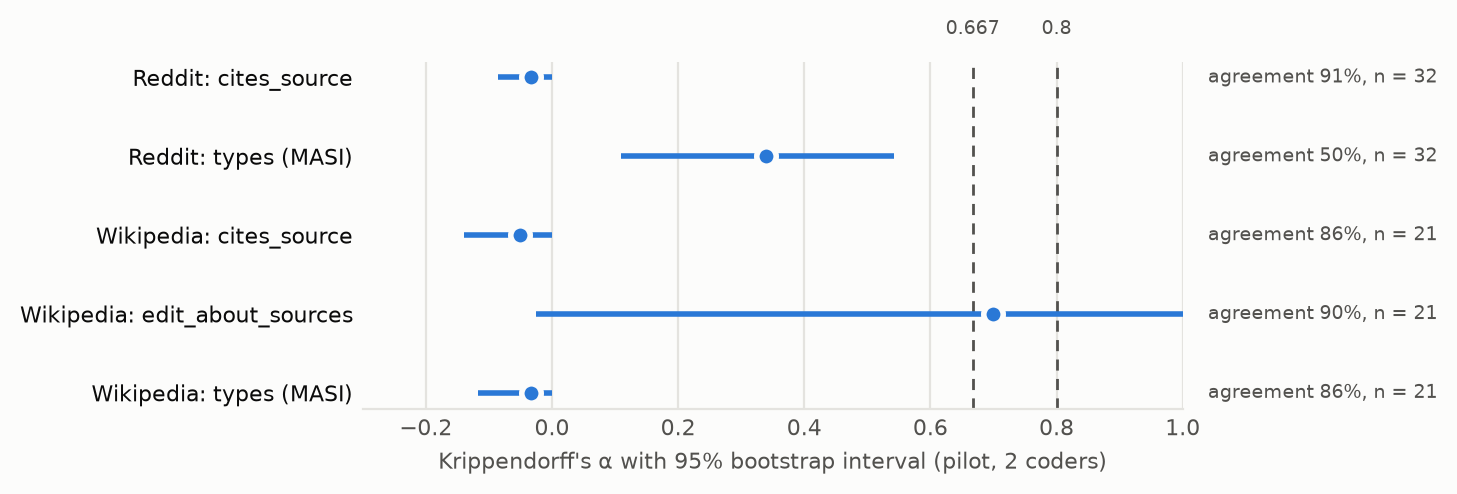
\includegraphics[width=0.85\linewidth]{preprint_agreement.png}
\caption{Agreement between the two annotators in the pilot: Krippendorff's $\alpha$ with 95\,\% intervals and the thresholds 0.667 and 0.8.}
\label{fig:agreement}
\end{figure}

\subsection{Blind AI Annotation Protocol}
To obtain annotations without new manual coding, and to test how reliable they are, we wrote a blind
annotation protocol. Before coding, the codebook and the protocol were frozen by recording their checksums,
and the batch of units was drawn with a fixed seed. Each unit received a random code and appeared in random
order, showing only the fields the human annotators had seen. The annotator was a large language model
(Claude Opus~5.5) run as a fresh agent with no project context. It received only the codebook, the protocol
and its batch, and it was not allowed to open links, browse the web or use programs to assign labels.
The key linking codes to units was kept outside the repository until the labels were frozen, and labels
were never changed afterwards. We checked the agents' transcripts for the files they accessed. Two runs
were interrupted by a usage limit and resumed with identical instructions. The agents' environment also
exposed the project's memory index, file names and commit titles, which we report as a limitation.

\subsection{Annotation Experiments and Their Measures}
E1 applied protocol~1.0 and codebook~2.2 to the 253 units coded by IS, in two independent runs (A and B).
E2 repeated the design with codebook~2.3 and protocol~1.1 (runs C and D). E3 coded the stance of the reference
posts in two independent runs (S1 and S2), each split between two agents. Stability between runs is
measured with Cohen's $\kappa$ for \kod{cites\_source}, \kod{edit\_about\_sources} and stance, and with
Krippendorff's $\alpha$ under the MASI distance for the set-valued \kod{source\_types}
\cite{cohen1960,krippendorff2004,passonneau2006}. Agreement with the reference is measured with F1,
sensitivity, specificity and MASI. Intervals for proportions are Wilson intervals; the others are
percentile bootstrap intervals over units (2000 draws). We pre-set three criteria: stability $\kappa \geq
0.8$ (K1); errors of the AI annotator and of each instrument should not coincide, $\kappa < 0.4$ between
their error indicators (K2); and sensitivity for \kod{challenges} $\geq 0.8$ (B2). In exploratory analyses
we compare paired runs with McNemar's test \cite{mcnemar1947} and relate errors to the annotator's own
uncertainty flag with Fisher's exact test.

\subsection{Instruments and Statistical Analysis}
\label{sec:instruments}
Three instruments were evaluated for source references: a rule-based baseline (v1) carried
over unchanged from the exploratory notebooks; a zero-shot classifier in which a
multilingual natural language inference (NLI) model scores one hypothesis per codebook
category; and GLiNER \cite{zaratiana2024}, which extracts mentions of sources and maps them
onto the codebook categories. Thresholds were tuned on the development split only, and the
instruments were frozen (commit \kod{33ff729}) before a single run on the test split. We
report F1 for \kod{cites\_source}, MASI agreement on the sets of source types
\cite{passonneau2006} and Cohen's $\kappa$ \cite{cohen1960}, weighted by the design
weights and with bootstrap intervals (Fig.~\ref{fig:instruments}, Table~\ref{tab:test}).

For stance, the instrument \kod{stance\_v1} had to reach F1 $\geq 0.5$ and $\kappa \geq 0.4$
for \kod{challenges} before H1-A could be tested. The secondary H1-B indicators had to reach
a Youden's $J$ above 0.2 in an audit.

Trends were estimated using weighted logistic regression, where the dependent variable
was a binary indicator at the post level, and the predictors included year, measured from
the beginning of the study period, together with subreddit fixed effects. Consequently,
the annual odds ratio (OR) reflects change within subreddits rather than changes in sample
composition. Sampling weights (Section~\ref{sec:data}) were rescaled to have a mean of 1, and standard
errors were clustered by sampled day, which served as the sampling unit (534 clusters in
the main H1-B analysis). In accordance with the preregistration, a one-sided test in the
direction of the hypothesis ($\alpha = 0.05$) and 95\,\% confidence intervals were applied,
while secondary indicators were reported without adjustment for multiple testing.
An OR below 1 indicates a decline, whereas a one-sided $p$-value close to 1 indicates an
estimate in the direction opposite to the hypothesis. Annual proportions presented in
Fig.~\ref{fig:h1} are weighted and shown with 95\,\% bootstrap confidence intervals.

H2 used a logistic regression of the same form on added links, with article fixed effects
and errors clustered by revision (Section~\ref{sec:h2}). Because alternative links are rare,
robustness checks include Firth's penalised logit \cite{firth1993,heinze2002}, an exact
conditional test and a permutation test. Instrument error was corrected with the known
sensitivity and specificity \cite{rogan1978}. Changes in pooled shares were decomposed into
within-community change and composition \cite{kitagawa1955}.

\subsection{Power with Measurement Error}
An instrument with sensitivity $Se$ and specificity $Sp$ reports a share $p_{obs} = Se\,p + (1-Sp)(1-p)$
instead of the true share $p$. It flattens a logistic trend $\beta$ to
$\beta_{obs} = (Se+Sp-1)\,\beta\,p(1-p)/\{p_{obs}(1-p_{obs})\}$. With $N$ units spread over years with
variance $\mathrm{var}(t)$ and a design effect $\mathrm{DEFF}$ from clustering \cite{kish1965}, the test
statistic is approximately
\begin{equation}
z \approx \beta_{obs}\sqrt{N\,p_{obs}(1-p_{obs})\,\mathrm{var}(t)/\mathrm{DEFF}},
\end{equation}
and power is $\Phi(z - z_{1-\alpha})$. We checked the formula against simulation. Planning values came from
Study~1 without estimating any trend: base shares, instrument error rates and design effects. The design
effect was \resEPowerDeffHOne{} for H1 (implied by the Study~1 standard error) and \resEPowerDeffHTwo{} for
H2 once bulk revisions were excluded (\resEPowerDeffHTwoBulk{} with them).

\subsection{Hypothesis Ladders and the Power Gate}
\label{sec:ladders}
Because the original hypotheses may lack power, the draft amendment orders weaker variants of each
hypothesis into a ladder. The H1 ladder runs from the original within-community stance trend, through
alternative sources within communities (H1-S1) and in the whole discussion (H1-S2), to the share of
discussion in communities that question the consensus (H1-S3). The H2 ladder runs from the original
owner-based indicator, through the share of non-specialist sources (H2-S1) and a comparison of health and
control articles (H2-S2), to a bound on the share of alternative sources (H2-S4). Before the confirmatory
run, a power gate takes as primary test the first variant that passed its validity criteria and reaches a
power of at least 0.8 both to detect the SESOI and for TOST. The gate uses only nuisance values that reveal
no trend: units, error rates, pooled shares and design effects. The two primary tests are adjusted with
Holm's procedure \cite{holm1979}, and the secondary family separately. H2-S3 (faster removal of
non-specialist links) and H2-S5 (the share of alternative-by-domain links that lead to institutions)
are always secondary. TOST for trends measured by an instrument uses the bound flattened by
the instrument's error.

\section{Experiment and Results}
\label{sec:results}

\subsection{Experimental Pipeline}
The pipeline runs in seven stages, each implemented as a numbered script.
Data are downloaded from the Reddit archive and the Wikipedia API (scripts
00--01c), then sampled into frames and annotation sheets (02--06). Human and AI labels are collected and
merged (03--05, 26). The instruments are applied (07--08, 14), the hypotheses are tested (09--10, 16),
power is computed and the gate is applied (17, 27), and the results package is built (18, 24, 28). Three
points in the pipeline are frozen: the instruments' thresholds after tuning on \kod{dev}, the codebook and
protocol before each AI run, and the power gate before the confirmatory v2 run. Study~1 passes through all stages; experiments E1--E3 sit at
the labelling stage and E4 at the power stage. The main results are generated by the pipeline as \LaTeX{} macros;
descriptive counts of the raw data and the diagnostic power range in E4 are typed by hand.

\subsection{Study 1: Validation of the Instruments}
\label{sec:validation}

On Reddit, GLiNER performed best, with an F1 of \resTestGlinerRedditCitesF{} for
\kod{cites\_source} (recall \resTestGlinerRedditCitesRecall) and a MASI of
\resTestGlinerRedditMasi{} for source types, and was therefore chosen for H1-B.
In an exact McNemar test \cite{mcnemar1947}, GLiNER was right where the zero-shot
classifier erred in \resMcnemarRedditZeroshotGlinerOnlySecond{} posts and the reverse
occurred in \resMcnemarRedditZeroshotGlinerOnlyFirst{} ($p$ = \resMcnemarRedditZeroshotGlinerP),
and it also outperformed v1 ($p$ \resMcnemarRedditVoneGlinerP).
The baseline failed mainly because its rules ignore the link of a post, which accounts
for \resErrorsVoneUrl{} of its \resErrorsVoneTotal{} errors on the development split.
GLiNER's $\kappa$ for \kod{cites\_source} is only \resTestGlinerRedditCitesKappa{} despite
its high F1, because almost every post cites a source \cite{feinstein1990}.

On Wikipedia, no instrument performed adequately (GLiNER: F1 \resTestGlinerWikipediaCitesF),
so H2 is measured by the domains of added links (Section~\ref{sec:data}) rather than by a classifier.
The reference matters as well: on the units coded by IS, GLiNER's
MASI on Reddit was \resTestGlinerRedditMasiIS, against \resTestGlinerRedditMasiJP{} on the
units that JP coded. As these are different units, the gap
mixes the annotator, the pre-annotation and the units themselves, but the cleanest
reference yields clearly lower agreement on source types, so the overall value should be
read with caution.
GLiNER's false-positive rate on Reddit does not differ significantly over time
($p$ = \resDifferentialGlinerRedditPeriodFpP) but does differ between subreddits
($p$ = \resDifferentialGlinerRedditSubredditFpP, on few posts without a citation); subreddit
fixed effects absorb such constant differences, so only an error that changes over time
would bias the within-subreddit trends.

For stance (H1-A), \kod{stance\_v1} uses the same NLI model \cite{laurer2024} to score
whether a post concerns science, supports it or challenges the consensus. Its thresholds
were tuned on the development split (\resHoneADevPosts{} posts; \resHoneAThresholds),
frozen (commit \kod{7ad9409}) and applied once to \resHoneATestPosts{} test posts; an
enriched sample from r/conspiracy (\resEnrichedPosts{} posts with inclusion weights) raised
the number of test posts labelled \kod{challenges} to \resStanceTestChallengesPosts. The
reference is described in Section~\ref{sec:references}. On the \resHoneAReviewedPosts{} verified
test posts the instrument failed its validity criterion (F1 \resHoneATestChallengesF,
$\kappa$ \resHoneATestKappa): with a precision of \resHoneATestChallengesPrecision{} and a
recall of \resHoneATestChallengesRecall, the instrument is usually right when it flags a
post as challenging the consensus but misses most such posts (Fig.~\ref{fig:stance}).
On all \resHoneATestPosts{} test rows, $\kappa$ was \resHoneATestAllRowsKappa, and
performance on the development split was similar (F1 \resHoneADevChallengesF), so the
failure does not stem from overfitted thresholds.
A dry run of the pipeline on AI labels preceded this single test; the instrument and its
thresholds were not changed afterwards, and the dry run is recorded in the preregistration
log.

The audit of the H1-B indicators applied the preregistered criterion of Youden's $J$ above
0.2 on the audit sample and the gold test split combined (\resAuditConsensusPositives{} and
\resAuditAlternativePositives{} positive cases): consensus sources reached
$J$ = \resAuditConsensusJ{} (0.199 before rounding; sensitivity
\resAuditConsensusSensitivity) and are reported descriptively only, whereas alternative
sources are valid ($J$ = \resAuditAlternativeJ); Section~\ref{sec:h1} reads H1-B accordingly.

\begin{figure}[htbp]
\centering
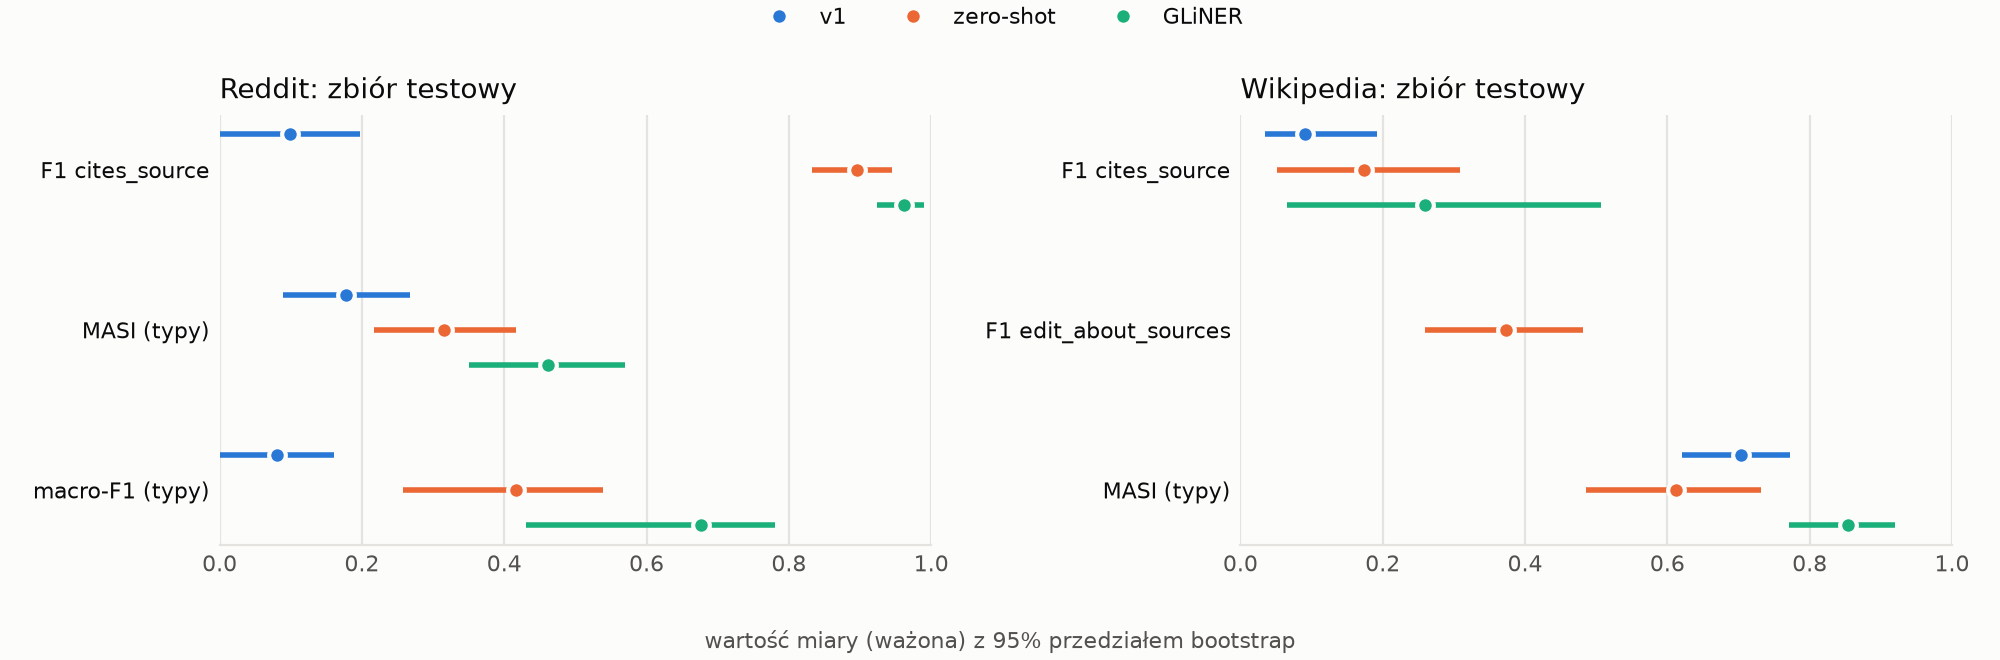
\includegraphics[width=\linewidth]{preprint_instruments.png}
\caption{Weighted test-set metrics of the three source instruments, with 95\,\% bootstrap intervals.}
\label{fig:instruments}
\end{figure}

\begin{table}[htbp]
\centering
\caption{Results on the test split (a single run of the frozen instruments).}
\label{tab:test}
\tabela{preprint_test_metrics}
\end{table}

\begin{table}[htbp]
\centering
\caption{Stance towards the scientific consensus (H1-A): quality of the reference (two-person agreement, rule R14, AI pre-annotation verified by \resPlanCCheckedBy) and results of \kod{stance\_v1}; preregistered validity criterion: F1 for \kod{challenges} $\geq$ 0.5 and $\kappa \geq$ 0.4 on the test split, on rows verified by \resPlanCCheckedBy.}
\label{tab:stance}
\tabela{preprint_stance}
\end{table}

\begin{figure}[htbp]
\centering
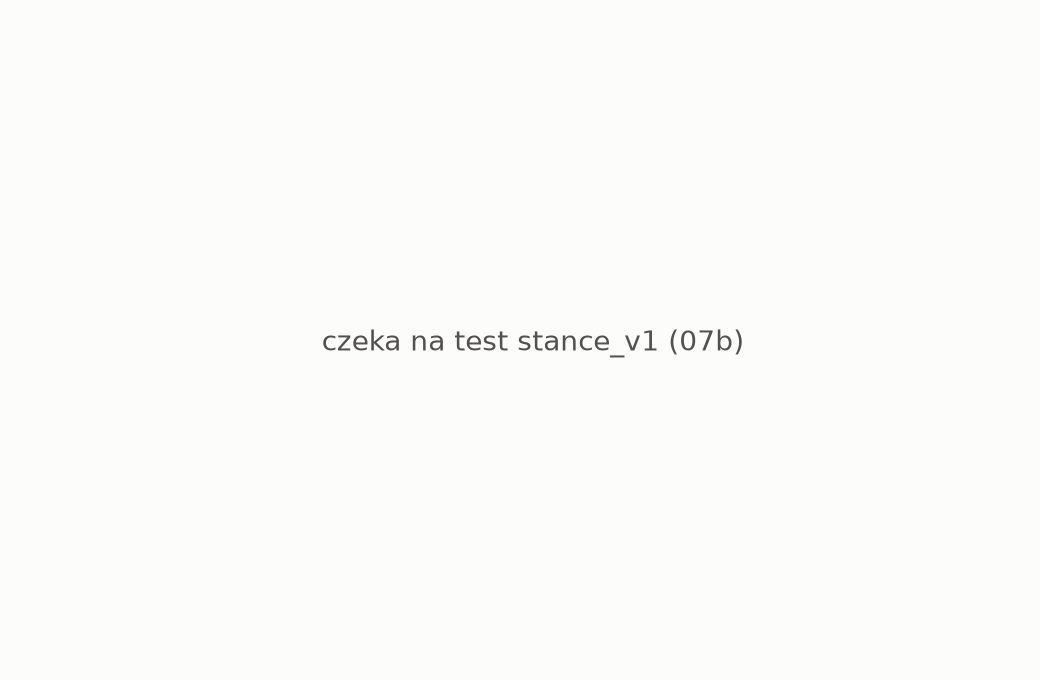
\includegraphics[width=0.6\linewidth]{preprint_stance_confusion.png}
\caption{Confusion matrix of \kod{stance\_v1} on the test split (gold and enriched sample): rows are the reference, columns the instrument.}
\label{fig:stance}
\end{figure}

\subsection{Study 1: Trust in the Scientific Consensus (H1)}
\label{sec:h1}

The primary H1 test (H1-A) was not conducted, because \kod{stance\_v1} failed its
validity criterion (Section~\ref{sec:validation}, Table~\ref{tab:stance}).
According to the decision rule specified prior to trend testing, H1-A was therefore not
estimated (Table~\ref{tab:h1}). This constitutes a negative result regarding measurement
validity and neither supports nor refutes H1. For such a contingency, the preregistration
specified a fallback test: the consensus-source indicator from H1-B was designated as the
confirmatory test for H1.

The H1-B indicators were estimated on \resHoneBCiting{} source-citing posts from
2005--2018, identified using the GLiNER instrument validated in Section~\ref{sec:validation}. The
consensus-source indicator did not satisfy its validity criterion (Section~\ref{sec:validation}).
Accordingly, this indicator is reported descriptively only, and the fallback testing
rule cannot be applied; as a consequence, H1 lacks a valid confirmatory test.
Descriptively, the share of consensus sources does not exhibit a decline within
subreddits (OR = \resHoneBConsensusOr, $p$ = \resHoneBConsensusP). The only valid
H1-B indicator is alternative sources ($J$ = \resAuditAlternativeJ), whose share
also shows no increase (OR = \resHoneBAlternativeOr,
$p$ = \resHoneBAlternativeP; Table~\ref{tab:h1}).
The upper confidence-limit bound is inconsistent with an increase in odds greater
than approximately 1\,\% per year; however, without an equivalence test, this does
not constitute evidence for the absence of change.

None of the three preregistered sensitivity analyses (2005--2020 period, only r/science
during 2006--2018, and only r/conspiracy during 2008--2018) indicate a trend in the
hypothesised direction; the smallest one-sided $p$-value is
\resHoneBConsensusConspiracyP{} (Table~\ref{tab:h1}). Over the 2005--2020 period,
the share of consensus sources within subreddits actually increases
(OR = \resHoneBConsensusTwentyOr), implying change in the direction opposite to the
hypothesis; however, because the validity criterion was not met, this result remains
purely descriptive.
The preregistered Rogan--Gladen correction for annual proportions adjusts proportions
linearly for measurement error. Consequently, for alternative sources it lowers the
estimated level without altering the temporal pattern, whereas for consensus sources
it yields uninformative intervals because the correction divides by a $J$ value close
to 0.2.

Nevertheless, the raw weighted proportions in the full sample change in the
hypothesised direction (Fig.~\ref{fig:h1}): the share of consensus sources declines
from \resHoneBConsensusShareTwothousandsix{} in 2006 to
\resHoneBConsensusShareLateLow--\resHoneBConsensusShareLateHigh{} during 2016--2018,
whereas the share of alternative sources increases from approximately
\resHoneBAlternativeShareTwothousandfive{} during 2005--2007 to
\resHoneBAlternativeShareLateHigh{} during 2016--2018. The year 2005 was excluded
for consensus sources because the sample for that year consisted exclusively of the
general subreddit r/reddit.com. At the same time, sample composition changes:
the weighted share of r/conspiracy among source-citing posts increases from
\resHoneConspiracyShareTwothousandeight{} in 2008 to
\resHoneConspiracyShareTwothousandeighteen{} in 2018, and in this subreddit
citations to consensus sources are less frequent, whereas citations to alternative
sources are more frequent, than in r/science. An exploratory decomposition
\cite{kitagawa1955} of the change in the share of alternative sources between
2005--2009 and 2014--2018 (\resHoneBAlternativeShiftTotal) attributes
\resHoneBAlternativeShiftComposition{} to compositional change and only
\resHoneBAlternativeShiftWithin{} to change within subreddits.
In summary, H1 lacks a valid confirmatory test, the valid secondary indicator does
not support the hypothesis, and the change observed in the overall sample is explained
by shifts in community composition rather than by transformations occurring within
communities themselves.

\begin{figure}[htbp]
\centering
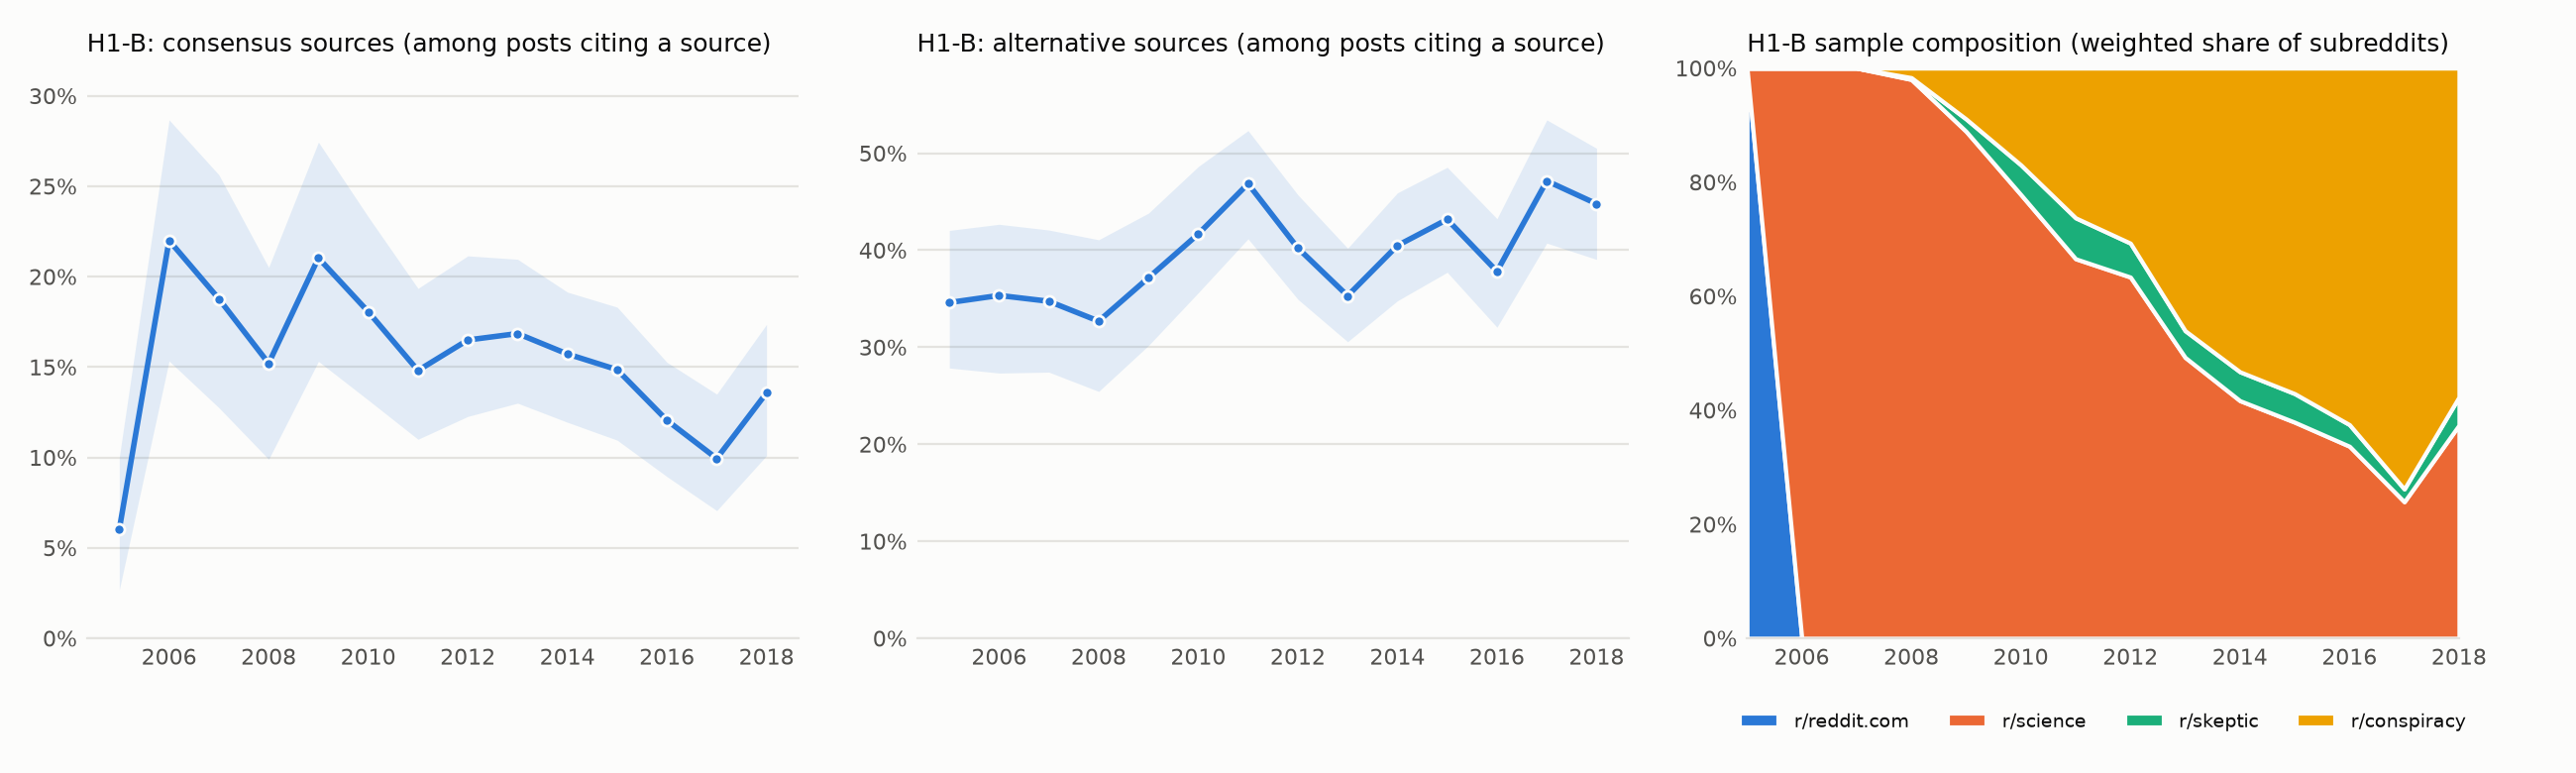
\includegraphics[width=\linewidth]{preprint_h1_en.png}
\caption{H1-B, 2005--2018: weighted yearly shares of consensus sources and of alternative sources among posts citing a source, with 95\,\% bootstrap intervals, and the weighted share of each subreddit in the sample.}
\label{fig:h1}
\end{figure}

\begin{table}[htbp]
\centering
\caption{H1: odds ratio per year [95\% CI] with subreddit fixed effects and one-sided $p$ in the hypothesised direction; H1-A is the primary test, H1-B the secondary indicators.}
\label{tab:h1}
\tabela{preprint_h1}
\end{table}

\subsection{Study 1: Alternative Sources in Wikipedia (H2)}
\label{sec:h2}

As preregistered, the share of alternative links among the \resHtwoLinks{} links added to
references in 2020--2026 (Section~\ref{sec:data}) was modelled by logistic regression on year with
article fixed effects, standard errors clustered by revision and a one-sided test; a link
counted as alternative when its domain belonged to the \kod{social\_blog} category (social
media, video platforms, blogs and newsletters), and no weights were needed, since all added
links were analysed. As the fixed effects drop articles without any alternative link, the
model uses \resHtwoModelLinks{} links from two articles, COVID-19 (1,102 links) and
Globalne ocieplenie (Global warming; 105 links), added in 180 revisions. The odds ratio per
year was \resHtwoOr{} ($p$ = \resHtwoP), meeting the preregistered criterion
(Table~\ref{tab:h2}), and it was identical before the manual review of the domain list
(OR = \resHtwoBeforeReviewOr, $p$ = \resHtwoBeforeReviewP), which changed no
\kod{social\_blog} domain.

The estimate rests on only \resHtwoAlternativeLinks{} alternative links in nine revisions
of \resHtwoAlternativePages{} articles, and the preregistered sensitivity analyses do not
reproduce it: without the COVID-19 article, OR = \resHtwoWithoutCovidOr{}
($p$ = \resHtwoWithoutCovidP), and without 2020, OR = \resHtwoWithoutTwentytwentyOr{}
($p$ = \resHtwoWithoutTwentytwentyP). The third analysis, restricted to classified domains,
coincides with the main test, because after the review every domain had a category.
Far fewer links were added in later years (780 in 2020, about 20 per year in 2024--2026),
so a single alternative link in 2025 already yields a share of 4.8\,\%; as the
preregistration anticipated, the test has very low power.

A reading of all ten alternative links, which was not preregistered and therefore qualifies
rather than replaces the test, shows that \resHtwoOfficialLinks{} of them lead to official
accounts of public health institutions in the COVID-19 article (Fig.~\ref{fig:h2}): a World
Health Organization livestream on Periscope, added \resHtwoWhoRepeats{} times because it
was restored after reverts, and a post of the Polish Chief Sanitary Inspectorate (GIS) on
Twitter, added twice. Only two links, both in Globalne ocieplenie, are alternative in the
sense of H2: a video on \kod{video.google.com} (2021) and a post on George Monbiot's blog
(2025). Classified by account owner, these \resHtwoByOwnerLinks{} links show no trend: an
exact conditional test, comparing their year sum with that of every pair of links in the
article, gives $p$ = \resHtwoExactP, and Firth's penalised logistic regression
\cite{firth1993} agrees (OR = \resHtwoOwnerOr, $p$ = \resHtwoOwnerP). Re-additions alone
do not explain the result: counting only the first addition of each link leaves a
borderline estimate (OR = \resHtwoFirstOr, $p$ = \resHtwoFirstP; \resHtwoFirstEvents{}
events). In the Firth models, $p$ and the interval come from the same profile penalised
likelihood \cite{heinze2002}, so a one-sided $p$ just below 0.05 is compatible with a
95\,\% interval that includes 1. The main test is also fragile, as permuting years across
revisions within articles gives $p$ = \resHtwoPermutationP.
Firth's model fitted to all articles gives OR = \resHtwoFirthOr{} ($p$ = \resHtwoFirthP).
Removing either of two links added in 2023, or the link added in 2025, lifts the $p$-value
of the preregistered model above 0.05, and the share of established sources, which should
fall if H2 held, does not decline (OR = 0.99, $p$ = 0.45).

H2 is therefore formally
supported, because the preregistered test met its criterion and the indicator may not be
redefined after seeing the data. Substantively, however, the result is an artefact of
classifying sources by domain, which does not separate an institution's account from an
alternative publisher, and of counting re-added links repeatedly; it does not show that
Wikipedia editors increasingly cite alternative sources.

\begin{figure}[htbp]
\centering
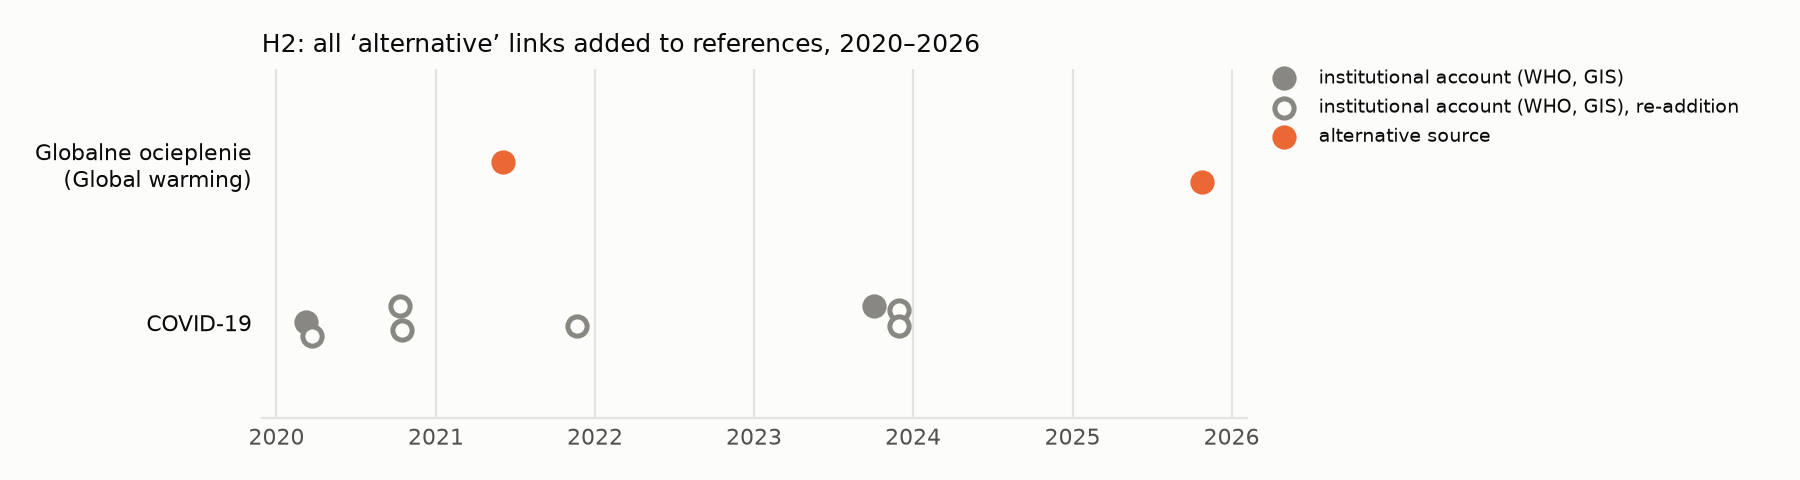
\includegraphics[width=\linewidth]{preprint_h2.png}
\caption{H2: all links classified as alternative by domain, by date and article, coloured by account owner; hollow markers are re-additions of the same link.}
\label{fig:h2}
\end{figure}

\begin{table}[htbp]
\centering
\caption{H2: preregistered test and sensitivity analyses, and exploratory analyses including the measurement check. In the Firth rows, $p$ and the interval come from the same profile penalised likelihood, without clustering by revision; the exact test is conditional on the article.}
\label{tab:h2}
\tabela{preprint_h2}
\end{table}

\subsection{E1--E2: AI Annotation of Sources}
The AI annotator was stable. Between runs A and B, $\kappa$ for \kod{cites\_source} was
\resESrcABCitesKappa; between C and D it was \resESrcCDCitesKappa, with $\alpha$ (MASI)
\resESrcCDTypesAlphaMasi{} for \kod{source\_types} and $\kappa$ \resESrcCDEditKappa{} for
\kod{edit\_about\_sources}. All lower bounds exceed 0.8, so K1 is met. For detecting a citation, agreement with IS
differed sharply between platforms (Tab.~\ref{tab:sources}, Fig.~\ref{fig:sources}). On Reddit it was high already under
codebook 2.2 (F1 \resESrcARedditFOne). On Wikipedia it was low (F1 \resESrcAWikipediaFOne), because the AI
missed \resESrcAWikipediaMissed{} citations that IS coded, mostly edit summaries that IS coded as an
opinion or an encyclopedic link. Under codebook 2.3, F1 on Wikipedia rose to \resESrcCWikipediaFOne{}, the
number of missed citations fell to \resESrcCWikipediaMissed{}, and $\kappa$ for \kod{personal} rose from
\resESrcAPersonalKappa{} to \resESrcCPersonalKappa. On source types the pattern is reversed: under codebook
2.3, MASI was \resESrcCRedditMasi{} on Reddit and \resESrcCWikipediaMasi{} on Wikipedia.

This gain is in-sample. The 2.3 rules were chosen to match IS's reading of the same 253 units, so they
show that the gap is a matter of definition, not that the AI generalises better. The paired comparison
supports this caution (exploratory): from A to C, \resESrcMcnemarACFixed{} units were fixed and
\resESrcMcnemarACBroken{} broken (McNemar $p$ = \resESrcMcnemarACP); from B to D, $p$ = \resESrcMcnemarBDP.
The new rules also changed the labels themselves ($\kappa$ between the 2.2 and 2.3 runs
\resESrcCodebookShiftKappaMin--\resESrcCodebookShiftKappaMax). K2 was met for the rules and the zero-shot
classifier, but not for GLiNER on either platform. The errors of the AI and of GLiNER therefore overlap, and
the AI cannot serve as an independent check of GLiNER.

\begin{table}[htbp]
\centering
\caption{E1--E2: agreement of the AI annotation runs with the labels of IS (coded without AI), with 95\,\% bootstrap intervals. Codebook 2.3 adopted IS's reading of the same units, so the gain of runs C and D is in-sample.}
\label{tab:sources}
\szeroka{v2_sources_runs}
\end{table}

\begin{figure}[htbp]
\centering
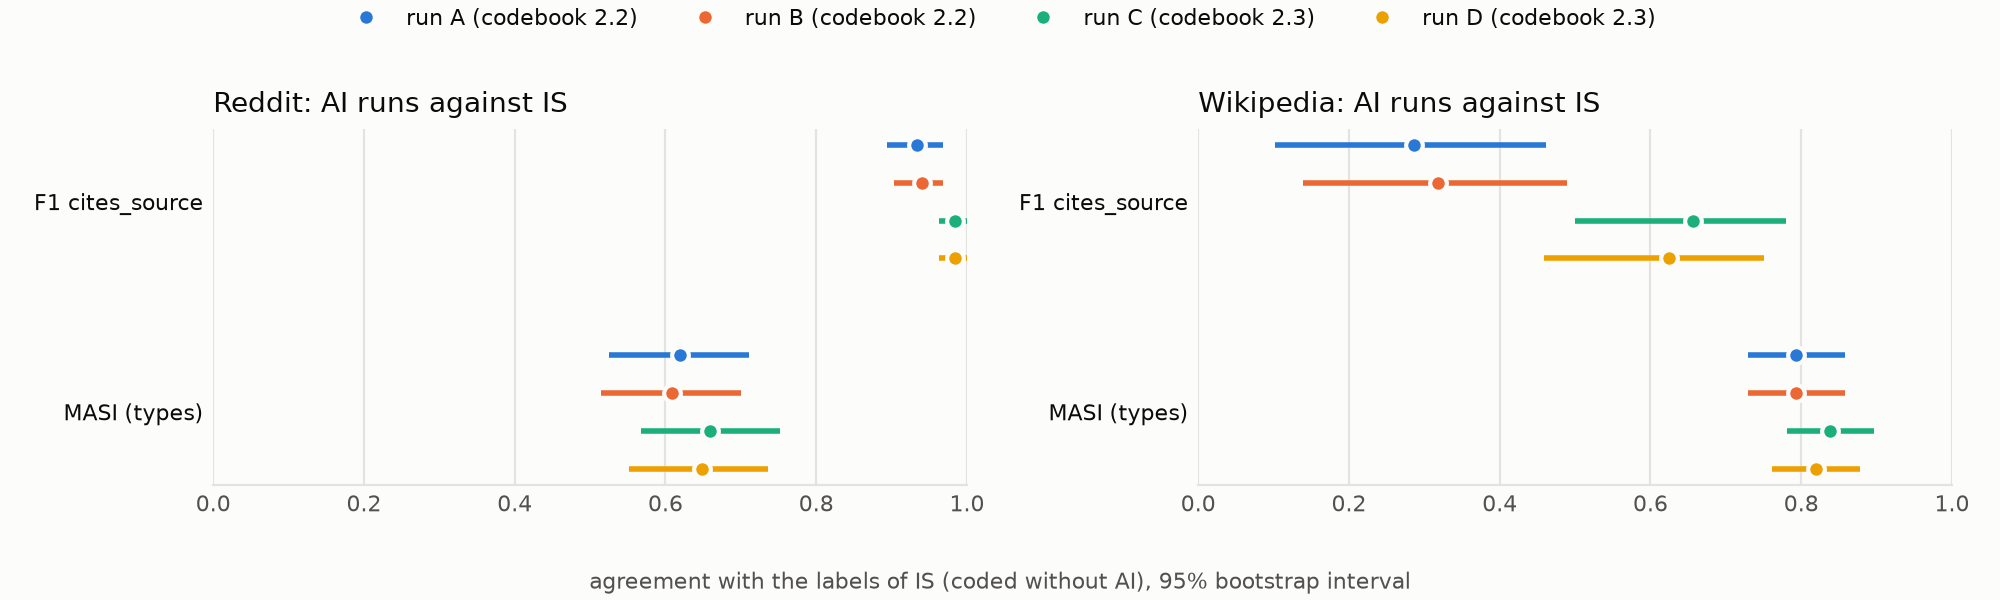
\includegraphics[width=\linewidth]{v2_sources_runs.png}
\caption{E1--E2: F1 of \kod{cites\_source} and MASI of \kod{source\_types} against IS for runs A--D, with 95\,\% bootstrap intervals.}
\label{fig:sources}
\end{figure}

\subsection{E3: AI Annotation of Stance}
The two stance runs agreed on \resEStanceAgreement{} of posts ($\kappa$ \resEStanceKappa). On the
\resEStanceAgreedUnits{} posts where they agreed, against the stance reference
(Tab.~\ref{tab:stance-ai}, Fig.~\ref{fig:stance-ai}), sensitivity for \kod{challenges} was
\resEStanceAgreedSensitivity, specificity \resEStanceAgreedSpecificity, F1 \resEStanceAgreedFOne{} and
$\kappa$ \resEStanceAgreedKappa. This is far above \kod{stance\_v1}. B2 is met only as a point estimate:
a test of sensitivity above 0.8 gives $p$ = \resEStanceAgreedBTwoP. The dominant error was coding a
challenge as \kod{neutral} (\resEStanceSOneChallengesAsNeutral{} posts in S1,
\resEStanceSTwoChallengesAsNeutral{} in S2). All four agents independently reported the same tension in
rule R14, which asks to code reported doubts as neutral. In an exploratory analysis, errors concentrated
in posts the annotator itself flagged as \kod{uncertain}: \resEStanceSOneErrorsFlagged{} flagged posts
against \resEStanceSOneErrorsUnflagged{} unflagged ones (Fisher $p$ \resEStanceSOneFisherP). Because the
reference is not independent of AI, these values may overstate the validity of the AI annotator.

\begin{table}[htbp]
\centering
\caption{E3: AI stance labels against the stance reference (\resEStanceReferenceUnits{} posts, \resEStanceReferenceChallenges{} \kod{challenges}); 95\,\% Wilson intervals for sensitivity and specificity, bootstrap for F1 and $\kappa$. The reference is not independent of AI.}
\label{tab:stance-ai}
\szeroka{v2_stance}
\end{table}

\begin{figure}[htbp]
\centering
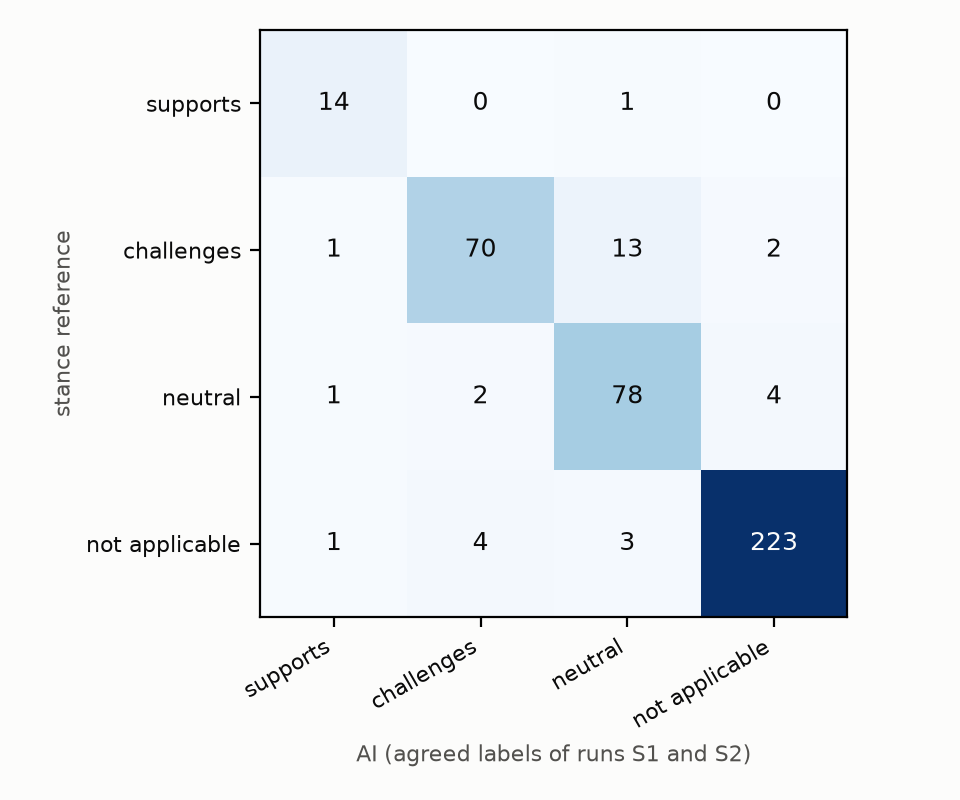
\includegraphics[width=0.55\linewidth]{v2_stance_confusion.png}
\caption{E3: agreed AI stance labels (runs S1 and S2 equal) against the stance reference.}
\label{fig:stance-ai}
\end{figure}

\subsection{E4: Power and the Power Gate}
Study~1 had little chance of settling its hypotheses. In an exploratory diagnostic at the smallest effect of
interest, fixed after Study~1, its power was only 0.11--0.43. Table~\ref{tab:power} and Fig.~\ref{fig:power} give the units needed for a power of 0.8,
with the instruments' error rates and the design effects of Study~1. With a stance instrument as good as
the AI annotator, H1 needs \resEPowerHOneTargetTenUnits{} units to detect the effect and
\resEPowerHOneTargetTenUnitsTost{} to show its absence. With \kod{stance\_v1} it would need
\resEPowerHOneStanceVOneUnits, so measurement matters more than data. The weaker variants need fewer units:
\resEPowerHOneSOneUnits{} for H1-S1 and \resEPowerHOneSThreeUnits{} for H1-S3. For H2 the owner-based
indicator is practically untestable at a base share of \resEPowerAltOwnerShare{}
(\resEPowerHTwoOwnerUnits{} links). The share of non-specialist sources (H2-S1) needs
\resEPowerHTwoSOneUnits. Applied to planning values only, the gate would choose \resEGatePlanHOnePrimary{}
as the primary test of H1 with \resEGatePlanHOneUnits{} units and \resEGatePlanHTwoPrimary{} for H2 with
\resEGatePlanHTwoLinks{} links. This is an illustration; the binding choice will be made on v2 nuisance
values.

\begin{table}[htbp]
\centering
\caption{E4: units needed for a power of 0.8 to detect the smallest effect of interest and to show its absence (TOST), with instrument error and the design effect of v1 (planning values; no v2 data).}
\label{tab:power}
\szeroka{v2_power}
\end{table}

\begin{figure}[htbp]
\centering
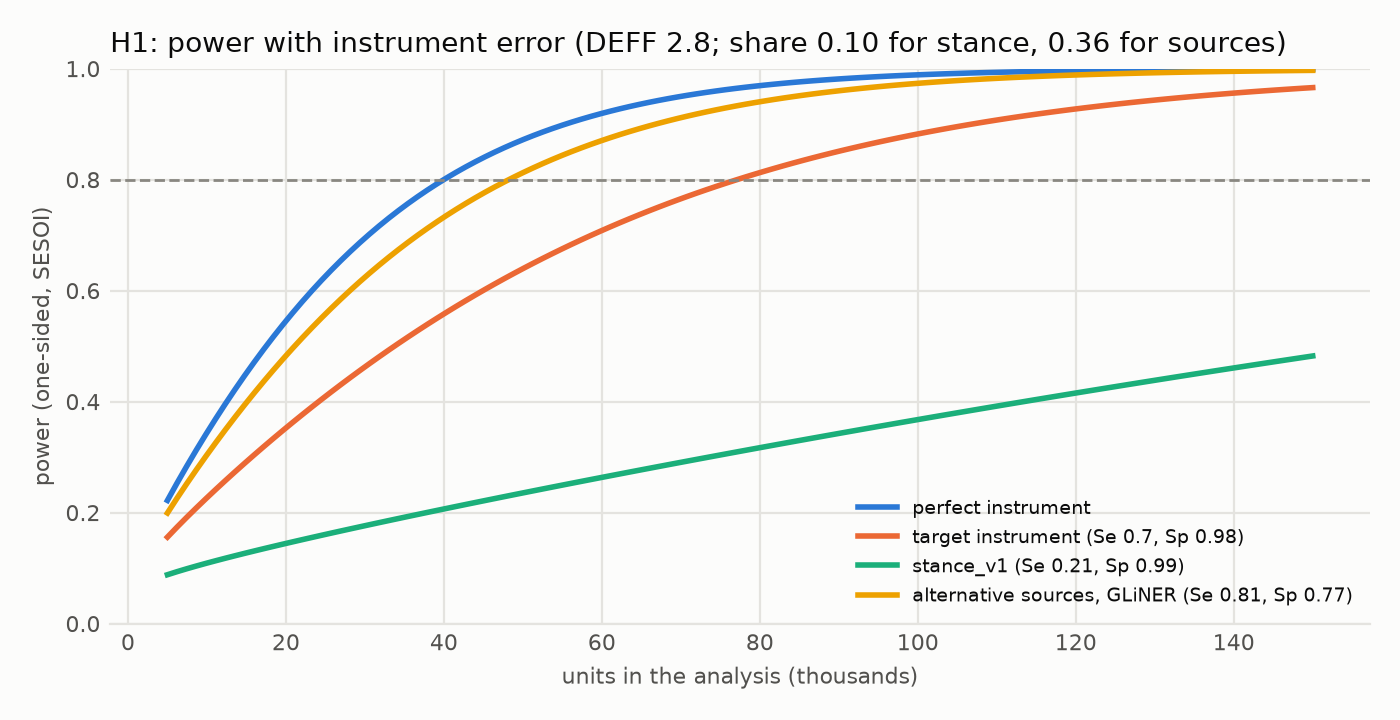
\includegraphics[width=0.85\linewidth]{v2_power.png}
\caption{E4: power of the H1 trend test against the number of units, by instrument (planning values).}
\label{fig:power}
\end{figure}

\subsection{Contradiction Analysis}
Three apparent contradictions run through the results. First, H2 is formally confirmed ($p$ = \resHtwoP)
but fails every check that classifies sources by owner ($p$ = \resHtwoExactP). The significant trend is an
artefact of a domain rule that counts official institutions' social media accounts as alternative.
Second, the AI agrees with IS on detecting citations on Reddit but not on Wikipedia. Since the gap
narrows once the rules are clarified (E2, F1 \resESrcCWikipediaFOne, an in-sample gain), it reflects at least
partly the definition of a citation in edit summaries rather than random error, although a gap remains.
Third, the stance runs are highly stable ($\kappa$ \resEStanceKappa) while sensitivity is
only \resEStanceAgreedSensitivity: two runs can agree on the same mistake, so stability is not validity.

\subsection{Status of the v2 Confirmatory Study}
The code for v2 is complete: the sampling frames, hypothesis ladders, power gate and decision rule with
Holm's adjustment. The amendment that introduces them is in draft. Before the confirmatory run, the team
must approve and commit the amendment, download the v2 data, label it, validate the instruments, and
commit the gate's decision. The run itself is then performed once. It has not been run, so this
article contains no v2 results. We fix the interpretations in advance. A confirmed primary variant supports
only that variant's weaker claim, not the original hypothesis. ``Refuted: no trend'' means that any change
is smaller than the SESOI. ``Inconclusive'' means that even the best-powered variant could not settle the
question with the available data.

\section{Conclusion}
\label{sec:conclusion}

\subsection{Summary}
We asked whether trust in science declined on Reddit and whether Polish Wikipedia editors turned to
alternative sources, and we found that the answer depends first on measurement. A blind AI annotation
protocol produced highly stable labels for sources ($\kappa$ \resESrcCDCitesKappa) and stance
($\kappa$ \resEStanceKappa). Part of its disagreement with a human coder came from the codebook's rules, although a gap remains after
the rules were clarified. In Study~1, H1 could not be tested because the stance classifier was not valid; the
only valid secondary indicator does not rise within subreddits, and the shift in the pooled sample is a
composition effect, as the growing share of r/conspiracy accounts for
\resHoneBAlternativeShiftComposition{} of the \resHoneBAlternativeShiftTotal{} change. The confirmation of H2
proved to be an artefact of how sources were classified: \resHtwoOfficialLinks{} of
\resHtwoAlternativeLinks{} links lead to official accounts. The power analysis shows that settling H1 needs both
a better instrument and tens of thousands of units. The owner-based H2 indicator is out of reach
(\resEPowerHTwoOwnerUnits{} links), whereas its weaker variant H2-S1 needs about \resEPowerHTwoSOneUnits. A power
gate, once approved, makes it possible to test weaker claims without choosing them after seeing the data.

\subsection{Discussion}
\label{sec:discussion}

The central question of H1 remains open. Its primary test could not be carried out
because the stance instrument did not meet the preregistered validity criterion, which
neither supports nor refutes the hypothesis, and the fallback indicator of consensus
sources failed its own criterion, so H1 has no valid confirmatory test. Since Study~1
included neither a power analysis nor an equivalence test, the absence of a detectable
trend in H1-B is not evidence that no change occurred; E4 shows how many units such
evidence would require.

The main lesson concerns measurement. Without validating the instruments and the
indicators, H2 would have been read as a shift towards alternative sources and the raw
decline of consensus sources as a sign of declining trust. First, a domain does not
identify the publisher: an institution's account on a social platform looks like an
alternative source, and a link restored after reverts is counted as added several times,
so the unit of analysis has to be checked on raw cases. Second, a changing mix of
communities can masquerade as a trend, so pooled trends should be decomposed into
composition and within-community change. Third, an AI instrument should not be validated
against labels derived from AI pre-annotations: on the units coded by IS without
pre-annotations, GLiNER's agreement on source types was \resTestGlinerRedditMasiIS,
against \resTestGlinerRedditMasiJP{} on the units coded by JP, a gap that, although it compares different units, suggests that such a
reference can flatter an instrument.
Finally, high precision is not enough to measure a trend: the stance instrument reached a
precision of \resHoneATestChallengesPrecision{} but a recall of only
\resHoneATestChallengesRecall, whereas a trend requires recall that is high and stable over
time. Automated measures therefore have to be validated anew for each application
\cite{grimmer2013}.

\subsection{Limitations}

We group the limitations by type of validity \cite{shadish2002}. \emph{Construct
validity:} the stance instrument and the consensus indicator do not measure their
constructs validly, domain-based classification conflates platforms with publishers, and
the sources people cite are only an indirect proxy for trust. \emph{Quality of the
reference:} the references for stance and for the audit of the H1-B indicators, like JP's labels in the gold standard, rest on AI pre-annotations verified by one person; every gold-standard unit was coded by a single annotator, so two-coder
agreement exists only for the pilot, whose second round was coded by one annotator and
whose disputed units were never adjudicated, and no two-person stance pilot was
conducted. The evaluation in Section~\ref{sec:validation} and the validity decisions for H1-B may thus be
biased in an unknown direction, although for source types the cleanest reference gives
lower agreement. \emph{Statistical conclusion validity:} H2 rests on
\resHtwoAlternativeLinks{} events in two articles, a dry run of the pipeline on AI labels
preceded the confirmatory test (disclosed in the preregistration log, with the instrument
and thresholds unchanged), and the measurement checks were defined after seeing the data.
\emph{Internal validity:} the trends are correlational, and subreddit fixed effects remove
differences between communities but not changes in their membership. \emph{External
validity:} the evidence comes from posts, without comments, in four English-language
subreddits and from eight purposively selected articles of the Polish Wikipedia, which
limits generalisation to the online space named in the hypotheses.
\emph{AI annotation:} the only reference independent of AI is small (253 units) and reflects
one person's reading; the gain of codebook 2.3 was measured on the units used to design it;
rule R14 is ambiguous; K2 is not met for GLiNER; and the agents' environment exposed project
metadata that a fully blind design would hide. The results of v2 do not exist yet.

\subsection{Future Work}

These limitations point to clear next steps. Pilot round 2 and resolution could be
completed. Independent double-coding, without pre-annotations, could be added for the
stance and audit references and for part of the gold standard. These labels would make
H1-A testable. A second preregistration (v2) was committed before any new data collection.
It measures stance on specific consensus topics, classifies sources by
account owner, counts only first additions, sizes both frames with a power analysis and adds
equivalence tests against a smallest effect size of interest (odds ratios 1.25 for H1 and 1.5
for H2).
The next steps are to approve the amendment and run v2 through the power gate; to clarify R14
in codebook 2.4 and validate the AI annotator on new units coded by people without AI; and to
apply measurement-error corrections such as prediction-powered inference
\cite{angelopoulos2023} to the trend estimates.

\subsection{Reproducibility, Data and Use of AI}
\label{sec:reproducibility}

Code, configuration, labels and results are available in the project
repository\footnote{\url{https://github.com/igor-sosnowicz/digital-media-analysis}}. The
environment is pinned, random seeds are
fixed. Data retrieval runs with
\kod{make pipeline} and the path from labels to the results package with
\kod{make finish-results}; the main results in the text are macros generated by
\kod{make preprint-package} and script 28. Power, the
AI protocol and the gate are reproduced with scripts 17, 26 and 27. The preregistration and its dated amendments are kept in
\kod{docs/hipotezy.md} (commit \kod{440b5fb}); the source instruments were frozen in
commit \kod{33ff729} and the stance instrument in \kod{7ad9409}, before their single
tests, and the follow-up preregistration (v2) was committed in \kod{f375df6}. Re-running
the retrieval may yield slightly different data, because the archive and Wikipedia change
over time; the repository therefore keeps the annotation sample with its design weights
and the labels, and the human coding steps are stored as label files rather than re-run.

Posts from ten subreddits were obtained from the Arctic Shift archive and the revision
histories of eight articles of the Polish Wikipedia through the MediaWiki API
(Section~\ref{sec:data}); no usernames, editor names or IP addresses were collected.  The repository
shares the texts of the annotation sample, so that the coding can be repeated, together
with the labels and results, but not the full sampling frames. Wikipedia content is
available under the CC BY-SA licence, and Reddit content is subject to the platform's user
agreement.
% Check before submission: whether Reddit's and Arctic Shift's terms allow sharing the post
% texts of the annotation sample, and how the CC BY-SA attribution of Wikipedia texts is given.

Two AI coding assistants, Claude (Anthropic) and OpenCode (with a Chinese model DeepSeek 4.1), supported the
project. The hypothesis tests of Study~1 used the local open models with pinned revisions
described in Section~\ref{sec:methodology}, not the assistants. AI nevertheless entered the
measurement in two ways: the assistant pre-annotated units later verified by JP, and Claude
Opus~5.5 was the blind annotator in E1--E3. At the team's request, the
assistants also wrote code, tests and analysis scripts, produced the results package (macros,
tables and figures) and drafted documentation, including the text of both preregistrations
and their amendments; commits prepared with them are marked as co-authored in the
repository history.
% Variant B (current state): keep while the drafts are not rewritten by the authors.
Drafts of the abstract and of all four sections, except the paragraphs on the gold-standard
and analysis samples in Section~\ref{sec:data}, were prepared by the assistant from the
authors' outlines and results and were revised by the authors.
% Variant A: use instead of variant B only if the authors rewrote all these drafts in their own words.
% The assistant prepared outlines of the sections; the text was written by the authors.
The authors checked the results and take responsibility for the content.

% Optional: author contributions (list only what each person actually did).
% \paragraph{Author contributions.} J.P.: [...]. I.S.: [...].

\begin{thebibliography}{99}
\bibitem{algan2021} Y.~Algan, D.~Cohen, E.~Davoine, M.~Foucault, S.~Stantcheva. Trust in scientists in times of pandemic: Panel evidence from 12 countries. \textit{PNAS}, 118(40):e2108576118, 2021.
\bibitem{angelopoulos2023} A.~N. Angelopoulos, S.~Bates, C.~Fannjiang, M.~I. Jordan, T.~Zrnic. Prediction-powered inference. \textit{Science}, 382(6671):669--674, 2023.
\bibitem{cohen1960} J.~Cohen. A coefficient of agreement for nominal scales. \textit{Educational and Psychological Measurement}, 20(1):37--46, 1960.
\bibitem{cologna2025} V.~Cologna et~al. Trust in scientists and their role in society across 68 countries. \textit{Nature Human Behaviour}, 9:713--730, 2025.
\bibitem{egami2023} N.~Egami, M.~Hinck, B.~M. Stewart, H.~Wei. Using imperfect surrogates for downstream inference: Design-based supervised learning for social science applications of large language models. In: \textit{Advances in Neural Information Processing Systems 36}, 68589--68601, 2023.
\bibitem{feinstein1990} A.~R. Feinstein, D.~V. Cicchetti. High agreement but low kappa: I.~The problems of two paradoxes. \textit{Journal of Clinical Epidemiology}, 43(6):543--549, 1990.
\bibitem{firth1993} D.~Firth. Bias reduction of maximum likelihood estimates. \textit{Biometrika}, 80(1):27--38, 1993.
\bibitem{fong2021} C.~Fong, M.~Tyler. Machine learning predictions as regression covariates. \textit{Political Analysis}, 29(4):467--484, 2021.
\bibitem{ford2013} H.~Ford, S.~Sen, D.~R. Musicant, N.~Miller. Getting to the source: Where does Wikipedia get its information from? In: \textit{Proceedings of WikiSym}, 1--10, 2013.
\bibitem{gauchat2012} G.~Gauchat. Politicization of science in the public sphere: A study of public trust in the United States, 1974 to 2010. \textit{American Sociological Review}, 77(2):167--187, 2012.
\bibitem{gilardi2023} F.~Gilardi, M.~Alizadeh, M.~Kubli. ChatGPT outperforms crowd workers for text-annotation tasks. \textit{PNAS}, 120(30):e2305016120, 2023.
\bibitem{grimmer2013} J.~Grimmer, B.~M. Stewart. Text as data: The promise and pitfalls of automatic content analysis methods for political texts. \textit{Political Analysis}, 21(3):267--297, 2013.
\bibitem{heinze2002} G.~Heinze, M.~Schemper. A solution to the problem of separation in logistic regression. \textit{Statistics in Medicine}, 21(16):2409--2419, 2002.
\bibitem{holm1979} S.~Holm. A simple sequentially rejective multiple test procedure. \textit{Scandinavian Journal of Statistics}, 6(2):65--70, 1979.
\bibitem{horvitz1952} D.~G. Horvitz, D.~J. Thompson. A generalization of sampling without replacement from a finite universe. \textit{Journal of the American Statistical Association}, 47(260):663--685, 1952.
\bibitem{kish1965} L.~Kish. \textit{Survey Sampling}. Wiley, 1965.
\bibitem{kitagawa1955} E.~M. Kitagawa. Components of a difference between two rates. \textit{Journal of the American Statistical Association}, 50(272):1168--1194, 1955.
\bibitem{krause2019} N.~M. Krause, D.~Brossard, D.~A. Scheufele, M.~A. Xenos, K.~Franke. The polls---Trends: Americans' trust in science and scientists. \textit{Public Opinion Quarterly}, 83(4):817--836, 2019.
\bibitem{krippendorff2004} K.~Krippendorff. \textit{Content Analysis: An Introduction to Its Methodology}. 2nd ed. Sage, 2004.
\bibitem{lakens2018} D.~Lakens, A.~M. Scheel, P.~M. Isager. Equivalence testing for psychological research: A tutorial. \textit{Advances in Methods and Practices in Psychological Science}, 1(2):259--269, 2018.
\bibitem{laurer2024} M.~Laurer, W.~van Atteveldt, A.~Casas, K.~Welbers. Less annotating, more classifying: Addressing the data scarcity issue of supervised machine learning with deep transfer learning and BERT-NLI. \textit{Political Analysis}, 32(1):84--100, 2024.
\bibitem{lewandowsky2012} S.~Lewandowsky, U.~K.~H. Ecker, C.~M. Seifert, N.~Schwarz, J.~Cook. Misinformation and its correction: Continued influence and successful debiasing. \textit{Psychological Science in the Public Interest}, 13(3):106--131, 2012.
\bibitem{mcnemar1947} Q.~McNemar. Note on the sampling error of the difference between correlated proportions or percentages. \textit{Psychometrika}, 12(2):153--157, 1947.
\bibitem{nosek2018} B.~A. Nosek, C.~R. Ebersole, A.~C. DeHaven, D.~T. Mellor. The preregistration revolution. \textit{PNAS}, 115(11):2600--2606, 2018.
\bibitem{pangakis2023} N.~Pangakis, S.~Wolken, N.~Fasching. Automated annotation with generative AI requires validation. arXiv:2306.00176, 2023.
\bibitem{passonneau2006} R.~Passonneau. Measuring agreement on set-valued items (MASI) for semantic and pragmatic annotation. In: \textit{Proceedings of LREC 2006}, 2006.
\bibitem{piccardi2020} T.~Piccardi, M.~Redi, G.~Colavizza, R.~West. Quantifying engagement with citations on Wikipedia. In: \textit{Proceedings of The Web Conference 2020}, 2365--2376, 2020.
\bibitem{proferes2021} N.~Proferes, N.~Jones, S.~Gilbert, C.~Fiesler, M.~Zimmer. Studying Reddit: A systematic overview of disciplines, approaches, methods, and ethics. \textit{Social Media + Society}, 7(2), 2021.
\bibitem{redi2019} M.~Redi, B.~Fetahu, J.~Morgan, D.~Taraborelli. Citation needed: A taxonomy and algorithmic assessment of Wikipedia's verifiability. In: \textit{Proceedings of The World Wide Web Conference}, 1567--1578, 2019.
\bibitem{rogan1978} W.~J. Rogan, B.~Gladen. Estimating prevalence from the results of a screening test. \textit{American Journal of Epidemiology}, 107(1):71--76, 1978.
\bibitem{rutjens2018} B.~T. Rutjens, S.~J. Heine, R.~M. Sutton, F.~van Harreveld. Attitudes towards science. \textit{Advances in Experimental Social Psychology}, 57:125--165, 2018.
\bibitem{shadish2002} W.~R. Shadish, T.~D. Cook, D.~T. Campbell. \textit{Experimental and Quasi-Experimental Designs for Generalized Causal Inference}. Houghton Mifflin, 2002.
\bibitem{steinsson2024} S.~Steinsson. Rule ambiguity, institutional clashes, and population loss: How Wikipedia became the last good place on the internet. \textit{American Political Science Review}, 118(1):235--251, 2024.
\bibitem{teblunthuis2024} N.~TeBlunthuis, V.~Hase, C.-H. Chan. Misclassification in automated content analysis causes bias in regression. Can we fix it? Yes we can! \textit{Communication Methods and Measures}, 18(3):278--299, 2024.
\bibitem{tornberg2023} P.~Törnberg. ChatGPT-4 outperforms experts and crowd workers in annotating political Twitter messages with zero-shot learning. arXiv:2304.06588, 2023.
\bibitem{vosoughi2018} S.~Vosoughi, D.~Roy, S.~Aral. The spread of true and false news online. \textit{Science}, 359(6380):1146--1151, 2018.
\bibitem{zaratiana2024} U.~Zaratiana, N.~Tomeh, P.~Holat, T.~Charnois. GLiNER: Generalist model for named entity recognition using bidirectional transformer. In: \textit{Proceedings of NAACL 2024}, 5364--5376, 2024.
\bibitem{ziems2024} C.~Ziems, W.~Held, O.~Shaikh, J.~Chen, Z.~Zhang, D.~Yang. Can large language models transform computational social science? \textit{Computational Linguistics}, 50(1):237--291, 2024.
\end{thebibliography}

\end{document}
